% Emacs settings: -*-mode: latex; TeX-master: "manual.tex"; -*-

\chapter{Beam optical components:
Arms, slits, collimators, and filters}
This chapter contains a number of optical components
that is used to modify the neutron beam in various ways,
as well as the ``generic'' component {\bf Arm}.
\index{Library!Components!optics}
\index{Optics|textbf}

\section{Arm: The generic component}
\label{s:arm}
\index{Optics!Point in space (Arm, Optical bench)}
\mcdoccomp{optics/Arm.parms}


The component \textbf{Arm} is empty; is resembles an optical bench
and has no effect on the xray.
The purpose of this component is only to provide a standard
means of defining a local coordinate system within the instrument definition.
Other components may then be
positioned relative to the \textbf{Arm} component
using the \MCX\ meta-language.
The use of \texttt{Arm} components in the instrument definitions
is not required but is recommended for clarity.
\textbf{Arm} has no input parameters.

The first Arm instance in an instrument definition may be changed into a
\verb+Progress_bar+(sec.~\ref{s:progress_bar}) component in order to display
simulation progress on the fly , and possibly save intermediate results.


\section{Slit: A beam defining diaphragm}
\label{slit}
\index{Optics!Slit}

%\component{Slit}{System}{$x_{\rm min}$, $x_{\rm max}$, $y_{\rm min}$, $y_{\rm max}$}{$r$, $p_{\rm cut}$}{}
\mcdoccomp{optics/Slit.parms}

The component {\bf Slit} is a very simple construction.
It sets up an opening at $z=0$, and propagates the neutrons
onto this plane (by the kernel call PROP\_Z0).
Neutrons within the slit opening are unaffected,
while all other neutrons
are discarded by the kernel call ABSORB.

By using {\rm Slit}, some neutrons contributing to the background
in a real experiment will be neglected.
These are the ones that scatter off the inner side
of the slit, penetrates the slit material,
or clear the outer edges of the slit.

The input parameters of {\bf Slit} are the four coordinates,
$(x_{\rm min}, x_{\rm max}, y_{\rm min}, y_{\rm max})$
defining the opening of the rectangle, or the radius $r$ of
a circular opening, depending on which parameters are specified.

The slit component can also be used to discard insignificant 
({\em i.e.}\ very low weight)
neutron rays, that in some simulations may be very abundant and therefore
time consuming. If the optional parameter $p_{\rm cut}$ is set, all
neutron rays with $p<p_{\rm cut}$ are ABSORB'ed.
This use is recommended in connection with {\bf Virtual\_output}.




\section{Beamstop: A photon absorbing area}
\label{beamstop}
\index{Optics!Beam stop}

\mcdoccomp{optics/Beamstop.parms}

The component \textbf{Beamstop} can be seen as the reverse of
the \textbf{Slit} component.
It sets up an area at the $z=0$ plane. Photons that hit the plane 
within this area are ABSORB'ed, while all others are unaffected.

By using this component, some photons contributing to the background
in a real experiment will be neglected.
These are the ones that scatter off the side
of the (real) beamstop, or penetrate the absorbing material.
Further, the holder of the beamstop is not simulated.

\textbf{Beamstop} can be either circular or rectangular.
The input parameters of \textbf{Beamstop} are either height and width $(x_{width},y_{height})$ or the four coordinates,
$(x_\mathrm{min}, x_\mathrm{max}, y_\mathrm{min}, y_\mathrm{max})$
defining the opening of a rectangle, or the radius $r$ of
a circle, depending on which parameters are specified.

If the "direct beam" (e.g. after a monochromator or sample) should not be
simulated, it is possible to emulate an ideal beamstop 
so that only the scattered beam is left;
without the use of \textbf{Beamstop}:
This method is useful for instance in the case where only photons 
scattered from a sample are of interest. 
The example below removes the direct beam and 
any background signal from other parts of the instrument
\begin{verbatim}
COMPONENT MySample=V_sample(...) AT (...)
EXTEND
%{
  if (!SCATTERED) ABSORB;
%}
\end{verbatim}


\section{Filter: A general absorption filter model}
\label{s:filter}
\index{Optics!Filter}
\mcdoccomp{optics/Filter.parms}

This component is a filter in the shape of a rectangular block or a general
shape defined by a set of polygons. Given an input file containing material
parameters. Neccessary parameters are nominal density and a parameterization of
the linear attenuation coefficient, $\mu$ as a function of wavelength (or
energy).

The model is very simple: Firstly the X-ray is traced to find intersection points between ray and filter (0 or 2).
If no intersection is found the x-ray is left untouched and nothing further happens.
Assuming the ray intersects the filter: Secondly, the path length d$l$ within the filter is computed.
Thirdly a $\mu = f(\lambda,\mathrm{material})$ is computed by interpolating in
a datafile, and the x-ray weight is adjusted according to
$p=p\exp(-\mathrm{d}l*\mu)$. The x-ray is left at the point where it exits the
filter block (the $2$nd intersection).

Example data files corresponding to all elements up to $Z=92$ are distributed with \MCX in the
\verb+MCXTRACE/data+ directory as \verb+*.txt+ files. These tables have been
extracted from the NIST FFAST~\cite{NIST-ffast} x-ray database.
To generate other datafiles from the same source a simple shell script:
\verb+MCXTRACE/data/get_xray_db_data+ is also distributed with \MCX
Running this script will connect to the NIST webiste and download a
\verb+.html+ file. This output must now be modified such that \verb+html+-tags
are removed and all header lines begin with $\#$

\subsection{Example}
\label{getNISTdata}
This is an example of how to download and generate datafiles for the \verb+Filter.comp+ and others.

The distributed tables have been extracted from the NIST x-ray database. To ease generation of more dtafiles
from the same source a simple shell script:\\
\verb+MCXTRACE/data/get_xray_db_data+\\
is also distributed with \MCX

Running this script will connect to the NIST webiste and download a \verb+.html+ file. This output must now be modified wuch that \verb+html+-tags
are removed and all header lines begin with $\#$.

\begin {verbatim}
 /usr/local/lib/mcxtrace/data/get_xray_db_data 3 output.dat
\end{verbatim}
where the second parameter (3) is the atom number of the material, for which we want to generate a datafile.
Now open the generated datafile (\verb+output.dat+) with your favourite text editor and make sure the file ends up looking like this
\tiny
\begin{verbatim}
#Li (Z 3)
#Atomic weight: A[r]  6.941000
#Nominal density: rho 5.3300E-01
#    σ[a](barns/atom) = [μ/ρ](cm^2 g^-1)  ×  1.15258E+01
#    E(eV) [μ/ρ](cm^2 g^-1) = f[2](e atom^-1)  ×  6.06257E+06
#    2 edges. Edge energies (keV):
#
#
#    K      5.47500E-02  L I    5.34000E-03
#
#Relativistic correction estimate f[rel] (H82,3/5CL) = -9.8613E-04,
#    -6.0000E-04 e atom^-1
#    Nuclear Thomson correction f[NT] = -7.1131E-04 e atom^-1
#
#━━━━━━━━━━━━━━━━━━━━━━━━━━━━━━━━━━━━━━━━━━━━━━━━━━━━━━━━━━━━━━━━━━━━━━━━━━━━━━━
#Form Factors, Attenuation and Scattering Cross-sections
#Z=3, E = 0.001 - 433 keV
#
#    E        f[1]         f[2]        [mu/rho]    [sigma/rho]  [mu/rho]   [mu/rho][K] lambda
#                                    Photoelectric Coh+inc      Total
#   keV        e atom^-1    e atom^-1   cm^2 g^-1   cm^2 g^-1   cm^2 g^-1   cm^2 g^-1  nm
5.233200E-03  9.08733E-01  0.0000E+00  0.0000E+00  2.3914E-07  2.3914E-07  0.000E+00  2.369E+02
5.313300E-03  8.59283E-01  0.0000E+00  0.0000E+00  2.5404E-07  2.5404E-07  0.000E+00  2.333E+02
5.334660E-03  8.03599E-01  0.0000E+00  0.0000E+00  2.5813E-07  2.5813E-07  0.000E+00  2.324E+02
5.366700E-03  8.56971E-01  1.0769E-01  1.2165E+05  2.6435E-07  1.2165E+05  0.000E+00  2.310E+02
.
.
.
3.788588E+02  3.00000E+00  3.9121E-08  6.2602E-07  8.4389E-02  8.4390E-02  6.123E-07  3.273E-03
4.050001E+02  3.00000E+00  3.3438E-08  5.0054E-07  8.2127E-02  8.2128E-02  4.895E-07  3.061E-03
4.329451E+02  3.00000E+00  2.8581E-08  4.0022E-07  7.9892E-02  7.9892E-02  3.913E-07  2.864E-03
\end{verbatim}
\normalsize
Please make sure you don't forget to remove the html-tags in the bottom of the file as well. In the future we will set
up a more streamlined way of doing this.


\newpage
\section{Collimator\_linear: The simple Soller blade collimator}
\label{collimator-linear}\index{Optics!Linear collimator}

%\component{Collimator\_linear}{System}{$x_{min}$, $x_{max}$, $y_{min}$, $y_{max}$, $L$, $\delta$}{}{}
\mcdoccomp{optics/Collimator_linear.parms}

{\bf Collimator\_linear} models a standard linear Soller blade collimator.
The collimator has two identical rectangular openings,
defined by the $x$ and $y$ values. Neutrons not clearing both
openings are ABSORB'ed.
The length of the collimator blades is denoted $L$, while
the distance between blades is called $d$.

The collimating effect is taken care of by employing an approximately
triangular transmission through the collimator of width (FWHM) $\delta$, 
which is given in arc minutes, {\em i.e.} $\delta=60$ is one degree.
If $\delta=0$, the collimating effect is disabled,
so that the component only consists of two rectangular apertures.

For a more detailed Soller collimator simulation,
taking every blade into account, it is possible to use
{\bf Channeled\_guide} with absorbing walls, 
see section~\ref{s:channeled_guide}.

\begin{figure}[h!]
  \begin{center}
    \psfrag{xmin}[c][c]{$x_{\rm min}$}
    \psfrag{xmax}[c][c]{$x_{\rm max}$}
    \psfrag{ymin}[c][c]{$y_{\rm min}$}
    \psfrag{ymax}[c][c]{$y_{\rm max}$}
    \psfrag{delta}[c][c]{$\delta$}
    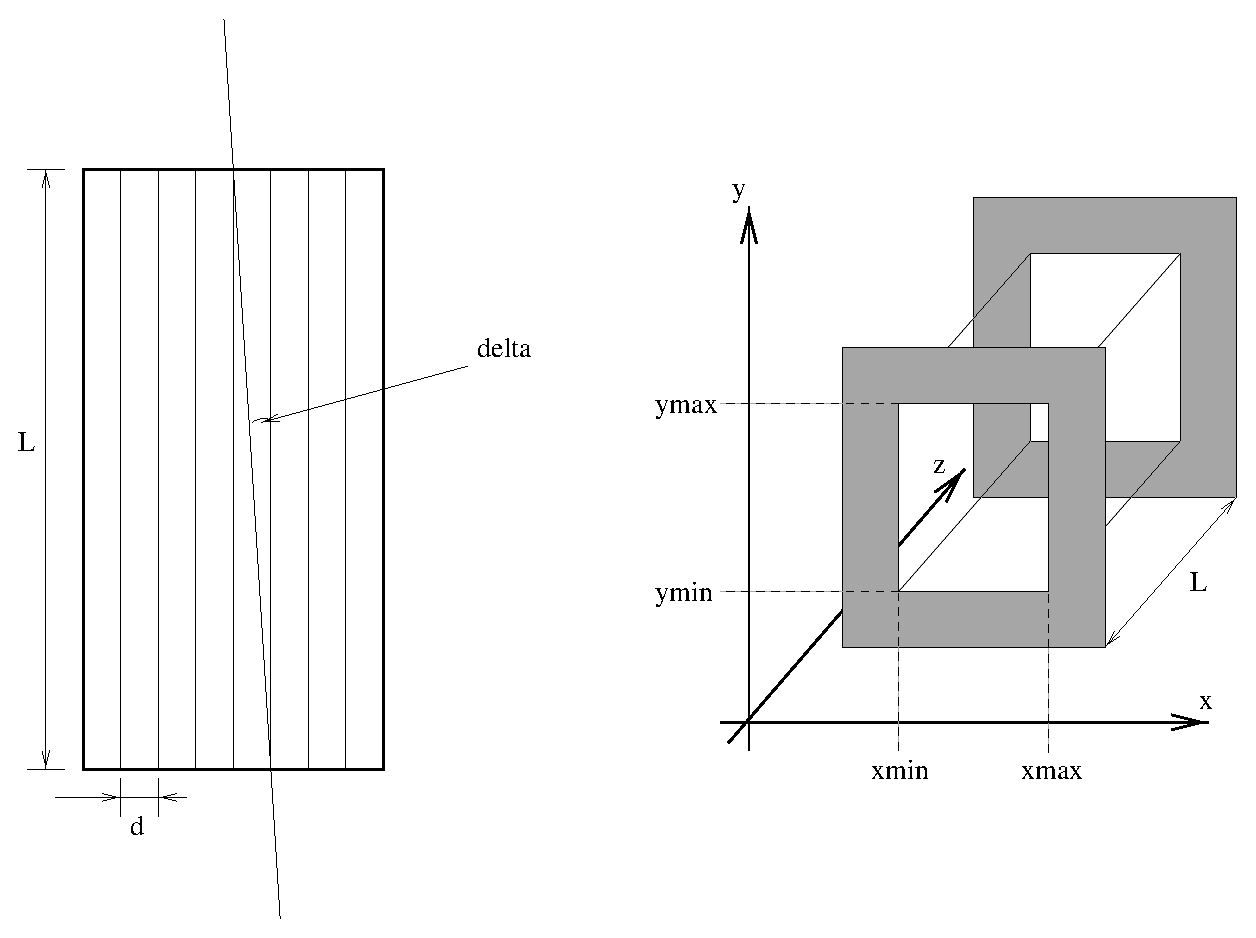
\includegraphics[width=0.7\textwidth]{figures/collimator}
  \end{center}
\caption{The geometry of a simple Soller blade collimators:
The real Soller collimator, seen from the top (left),
and a sketch of the component {\bf Soller} (right).
The symbols are defined in the text.}
\label{f:collimator}
\end{figure}

\subsection{Collimator transmission}
The horizontal divergence, $\eta_h$, is defined as the angle between the
neutron path and the vertical $y-z$ plane along the collimator axis.
We then define the collimation angle as the maximal allowed
horizontal divergence: $\delta = \tan^{-1}(d/L)$,
see Fig.~\ref{f:collimator}. Neutrons with a horizontal
divergence angle $|\eta_h| \geq \delta$ will always
hit at least one collimator blade and will thus be ABSORB'ed.
For smaller divergence angles, $|\eta_h| < \delta$, the fate of the
neutron depends on its exact entry point.
Assuming that a typical collimator has many blades, the
absolute position of each blade perpendicular to the collimator axis
is thus mostly unimportant.
A simple statistical consideration now shows that the transmission
probability is $T = 1-\tan|\eta_h|/\tan\delta$.
Often, the approximation $T \approx 1-|\eta_h|/\delta$ is used, giving
a triangular transmission profile.

\subsection{Algorithm}
The algorithm of {\rm Collimator\_linear} is roughly as follows:
\begin{enumerate}
\item Check by propagation if the neutron ray clear the entry and exit slits,
otherwise ABSORB.
\item Check if $|\eta_h| < \delta$, otherwise ABSORB.
\item Simulate the collimator transmission by a weight transformation:
\begin{equation}
\pi_i = T = 1-\tan|\eta_h|/ \tan\delta ,
\end{equation}
\end{enumerate}


\section{Collimator\_radial: A radial Soller blade collimator}
\index{Optics!Radial collimator}

\component{Collimator\_radial}{(System) E.Farhi, ILL}{$w_1$, $h_1$, $w_2$, $h_2$, $len$, $\theta_{min}$, $\theta_{max}$, $nchan$, $radius$}{$divergence$, $nblades$, $roc$ and others}{Validated}
%\mcdoccomp{optics/Collomator_radial.parms}

\begin{figure}
  \begin{center}
    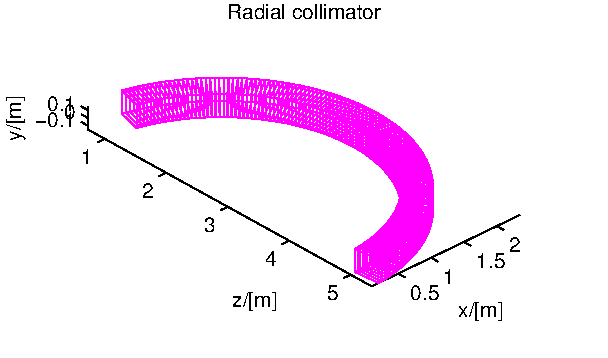
\includegraphics[width=0.8\textwidth]{figures/radial}
  \end{center}
\caption{A radial collimator}
\label{f:coll-radial}
\end{figure}

This radial collimator works either using an analytical approximation
like {\bf Collimator\_linear} (see section \ref{collimator-linear}),
or with an exact model.

The input parameters are the inner radius $radius$, the radial length $len$,
the input and output window dimensions $w_1$, $h_1$, $w_2$, $h_2$,
the number of Soller channels $nchan$
(each of them being a single linear collimator) covering the angular interval
[$\theta_{min}$, $\theta_{max}$] angle with respect to the $z$-axis.

If the $divergence$ parameter is defined,
the approximation level is used as in {\rm Collimator\_linear}
(see section \ref{collimator-linear}).
On the other hand, if you perfer to describe exactly the number of blades
$nblades$ assembled to build a single collimator channel,
then the model is exact, and traces the neutron trajectory inside each Soller.
The computing efficiency is then lowered by a factor 2.

The component can be made oscillating with an amplitude of $roc$ times
$\pm w_1$, which supresses the channels shadow.

As an alternative, you may use the {\bf Exact\_radial\_coll} contributed component.
For a rectangular shaped collimator, instead of cylindrical/radial, you may use the Guide\_channeled and the Guide\_gravity components.


\newpage
\chapter{Reflecting optical components: mirrors, and guides}
\index{Optics|textbf}

This section describes advanced neutron optical
components such as supermirrors and guides as well as various rotating choppers.
A description of the reflectivity of a supermirror is found
in section~\ref{s:mirror}.


\index{Optics|textbf}

This section describes advanced neutron optical
components such as supermirrors and guides.
A description of the reflectivity of a supermirror is found
in section~\ref{s:mirror}.

\section{Mirror: The single mirror}
\label{s:mirror}
\index{Optics!Mirror plane}
\component{Mirror}{System}{$l$, $h$, $m$}{$R_0, Q_c, W, \alpha, reflect$}{validated, no gravitation support}

The component {\bf Mirror}
models a single rectangular neutron mirror plate. It can be used
as a sample component or to \textit{e.g.}~assemble a complete neutron guide by putting multiple
mirror components at appropriate locations and orientations in the
instrument definition, much like a real guide is build from individual
mirrors.

In the local coordinate system, the mirror lies in the first quadrant of the
$x$-$y$ plane, with one corner at $(0,0,0)$.

The input parameters of this component are
the rectangular mirror dimensions $(l, h)$
and the values of $R_0, m, Q_c, W$, and $\alpha$ for the mirror reflectivity.
As a special case, if $m=0$ then the reflectivity is zero for all $Q$,
\textit{i.e.}\ the surface is completely absorbing.

This component may produce wrong results with gravitation.

\subsection{Mirror reflectivity}
\label{ss:mirrorreflect}
To compute the reflectivity of the supermirrors, we use an empirical
formula derived from experimental data \cite{pb_241_50},
see Fig.~\ref{f:reflectivity}. The reflectivity is given by
\begin{equation} \label{e:Rmirror}
  R = \left\{
    \begin{array}{ll}
      R_0 & \textrm{if $Q \leq Q_{\rm c}$} \\
      \frac{1}{2}R_0(1 - \tanh[(Q - m Q_{\rm c})/W])(1-\alpha(Q-Q_{\rm c}))
         & \textrm{if $Q > Q_{\rm c}$}
    \end{array}
  \right.
\end{equation}

Here $Q$ is the length of the scattering vector (in \AA$^{-1}$)
defined by
\begin{equation} \label{e:reflectivity}
Q = |{\bf k}_{\bf i} - {\bf k}_{\bf f}|
  = \frac{m_{\rm n}}{\hbar} |{\bf v}_{\bf i} - {\bf v}_{\bf f}|,
\end{equation}
$m_{\rm n}$ being the neutron mass.
The number $m$ in (\ref{e:Rmirror}) is a parameter determined by
the mirror materials,
the bilayer sequence, and the number of bilayers.
As can be seen, $R=R_0$ for $Q < Q_{\rm c}$, where $Q_{\rm c}$ is the
critical scattering wave vector for a single layer of the mirror
material. At higher values of $Q$, the reflectivity starts falling
linearly with a slope $\alpha$ until a "soft cut-off" at $Q = m Q_{\rm c}$.
The width of this cut-off is denoted $W$. See the example reflection curve in
figure~\ref{f:reflectivity}.

It is {\bf important} to notice that when $m < 1$, the reflectivity remains constant at $R=R_0$ up to $q=Qc$, and \emph{not} $m.Q_c$. This means that $m < 1$ parameters behave like $m=1$ materials.

Alternatively, the Mirror, Guide and Guide\_gravity components may use a reflectivity table $reflect$, which 1st column is q [$\AA^{-1}$] and 2nd column as the reflectivity $R$ in [0-1]. For this purpose, we provide $m=2$ and $m=3$ reflectivity files from SwissNeutronics (\verb+supermirror_m2.rfl+ and \verb+supermirror_m3.rfl+ in \verb+MCSTAS/lib/data/+).

\subsection{Algorithm}
The function of the component can be described as
\begin{enumerate}
\item Propagate the neutron ray to the plane of the mirror.
\item If the neutron trajectory intersects the mirror plate, it is
reflected, otherwise it is left untouched.
\item Reflection of the incident velocity
${\bf v}_{\rm i} = (v_x,v_y,v_z)$
gives the final velocity ${\bf v}_{\rm f} = (v_x,v_y,-v_z)$.
\item Calculate $Q=2 m_{\rm n} v_z / \hbar$.
\item The neutron weight is adjusted with the amount $\pi_i = R(Q)$.
\item  To avoid spending large amounts of computation time on very low-weight
neutrons, neutrons for which the reflectivity is lower than about
$10^{-10}$ are ABSORB'ed.
\end{enumerate}

\begin{figure}
  \begin{center}
    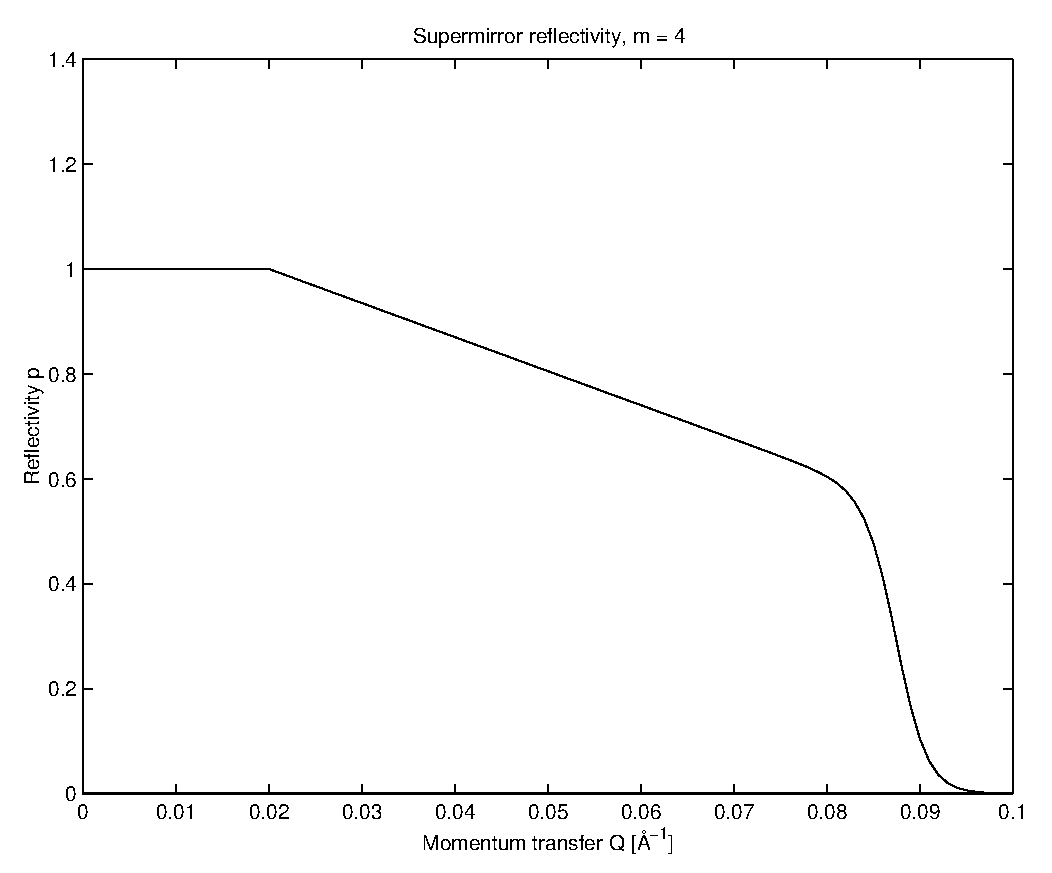
\includegraphics[width=0.6\textwidth]{figures/supermirror}
  \end{center}
\caption{A typical reflectivity curve for a supermirror,
Eq.~(\protect\ref{e:reflectivity}). The used values are
$ m=4$, $R_0=1$, $Q_{\rm c} = 0.02$~\AA$^{-1}$, $\alpha = 6.49$~\AA,
$ W=1/300$~\AA$^{-1}$.
}
\label{f:reflectivity}
\end{figure}

\newpage

\section{Guide: The guide section}
\index{Optics!Straight guide}

\component{Guide}{System}{$w_1, h_1$, $w_2, h_2$, $l$, $m$, $reflect$}{$R_0, Q_c, W, \alpha$}{validated, no gravitation support}

The component {\bf Guide}
models a guide tube consisting of four flat mirrors. The
guide is centered on the $z$ axis with rectangular entrance and exit
openings parallel to the $x$-$y$ plane. The entrance has the dimensions
$(w_1,h_1)$ and placed at $z=0$. The exit is of dimensions $(w_2,h_2)$
and is placed at $z=l$ where $l$ is the guide length. See
figure~\ref{f:guide}.
The reflecting properties are given by the values of
$R_0, m, Q_c, W$, and $\alpha$, as for {\bf Mirror}, or alternatively from the reflectivity file $reflect$.

{\bf Guide} may produce wrong results with gravitation support.
Use {\bf Guide\_gravity} (section \ref{s:guide_gravity}) in this case,
or the {\bf Guide\_channeled}
in section~\ref{s:channeled_guide}.

\begin{figure}
  \begin{center}
    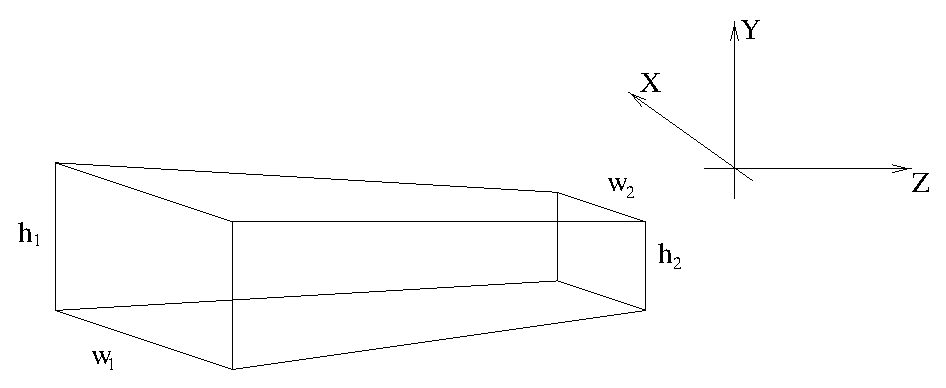
\includegraphics[width=0.7\textwidth]{figures/guide1}
  \end{center}
\caption{The geometry used for the guide component.}
\label{f:guide}
\end{figure}

\subsection{Guide geometry and reflection}
For computations on the guide geometry, we define the planes of the four
guide sides by giving their normal vectors (pointing into the guide)
and a point lying in the plane:
$$
\begin{array}{rclcrcl}
{\bf n}^v_1 &=& (l, 0, {(w_2 - w_1) / 2})
     & & {\bf O}^v_1 &=& (- w_1 / 2, 0, 0) \\
{\bf n}^v_2 &=& (-l, 0, {(w_2 - w_1) / 2})
     & & {\bf O}^v_2 &=& (w_1 / 2, 0, 0) \\
{\bf n}^h_1 &=& (0, l, {(h_2 - h_1) / 2})
     & & {\bf O}^h_1 &=& (0, - h_1 / 2, 0) \\
{\bf n}^h_2 &=& (0, -l, {(h_2 - h_1) / 2})
     & & {\bf O}^h_2 &=& (0, h_1 / 2, 0) \\
\end{array}
$$
In the following, we refer to an arbitrary guide side by its origin
{\bf O} and normal {\bf n}.

With these definitions, the time of intersection of the neutron with a
guide side can be computed by considering the projection onto the
normal:
\begin{equation}
t^\alpha_\beta = \frac{({\bf O}^\alpha_\beta - {\bf r}_0) \cdot {\bf n}^\alpha_\beta}
  {{\bf v} \cdot {\bf n}^\alpha_\beta}  ,
\end{equation}
where $\alpha$ and $\beta$ are indices for the different guide walls,
assuming the values (h,v) and (1,2), respectively.
For a neutron that leaves the guide directly through the guide exit we have
\begin{equation}
t_{\rm exit} = \frac{l - z_0}{v_z}
\end{equation}

The reflected velocity ${\bf v}_{\rm f}$ of the neutron with incoming velocity
${\bf v}_{\rm i}$ is computed by the formula
\begin{equation}
 {\bf v}_{\rm f} =
  {\bf v}_{\rm i}
   - 2{{\bf n} \cdot \frac{{\bf v}_{\rm i}}{{|{\bf n}|^2}} {\bf n}}
\end{equation}
This expression is arrived at by again considering the projection onto
the mirror normal (see figure~\ref{f:guidereflect}). The reflectivity of the
mirror is taken into account as explained in section~\ref{s:mirror}.

\begin{figure}
  \begin{center}
    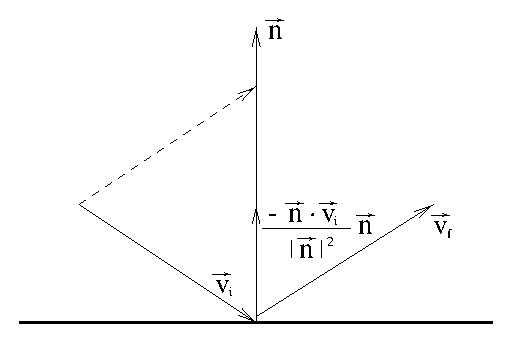
\includegraphics[width=0.5\textwidth]{figures/guide2}
  \end{center}
\caption{Neutron reflecting from mirror. ${\bf v}_{\rm i}$ and
${\bf v}_{\rm f}$ are the initial and final velocities, respectively,
and {\bf n} is a vector normal to the mirror surface.}
\label{f:guidereflect}
\end{figure}

\subsection{Algorithm}
\begin{enumerate}
\item The neutron is initially propagated to the $z = 0$ plane of the
guide entrance.
\item If it misses the entrance, it is ABSORB'ed.
\item Otherwise, repeatedly compute the time of intersection with the
four mirror sides and the guide exit.
\item The smallest positive $t$ thus
found gives the time of the next intersection with the guide (or in the
case of the guide exit, the time when the neutron leaves the guide).
\item Propagated the neutron ray to this point.
\item Compute the reflection from the side.
\item Update the neutron weight factor by the amount $\pi_i = R(Q)$.
\item Repeat this process until the neutron leaves the guide.
\end{enumerate}

There are a few optimizations possible here to avoid redundant
computations. Since the neutron is always inside the guide during the
computations, we always have
$({\bf O} - {\bf r}_0) \cdot {\bf n} \leq 0$.
Thus $t \leq 0$ if ${\bf v} \cdot {\bf n} \geq 0$, so in this case
there is no need to actually compute $t$. Some redundant computations
are also avoided by utilizing symmetry and the fact that many
components of {\bf n} and {\bf O} are zero.

\newpage

\section{Guide\_channeled: A guide section component with multiple channels}
\label{s:channeled_guide}
\index{Optics!Guide with channels (straight, non focusing)}

\component{Guide\_channeled}{System}{$w_1, h_1$, $w_2, h_2$, $l$, $k$, $m_x, m_y$}{$d, R_0, Q_{cx}, Q_{cy}, W, \alpha_x, \alpha_y$}{validated, no gravitation support}

The component {\bf Guide\_channeled} is a more complex variation of {\bf Guide}
described in the previous section. It allows the specification
of different supermirror parameters for the horizontal and vertical
mirrors, and also implements guides with multiple channels as used in
neutron bender devices. By setting the $m$ value of the supermirror
coatings to zero, nonreflecting walls are simulated;
this may be used for a very detailed simulation of a Soller collimator,
see section~\ref{collimator-linear}.

The input parameters are $w_1$, $h_1$, $w_2$, $h_2$, and $l$
to set the guide dimensions as for {\bf Guide}
(entry window, exit window, and length);
$k$ to set the number of channels; $d$ to set the thickness of the
channel walls; and $R_0$, $W$, $Q_{cx}$, $Q_{cy}$, $\alpha_x$, $\alpha_y$,
$m_x$, and $m_y$ to set the supermirror parameters as described under {\bf Guide}
(the names with \textit{x} denote the vertical mirrors,
and those with \textit{y} denote the horizontal ones).

\subsection{Algorithm}
The implementation is based on that of {\bf Guide}.
\begin{enumerate}
\item Calculate the channel which the neutron will enter.
\item Shift the $x$ coordinate so that the channel can be simulated
as a single instance of the {\bf Guide} component.
\item (do the same as in {\bf Guide}.)
\item Restore the coordinates when the
neutron exits the guide or is absorbed.
\end{enumerate}

\subsection{Known problems}\index{Bugs}
\begin{itemize}
\item This component may produce wrong results with gravitation support.
Use Guide\_gravity (section \ref{s:guide_gravity}) in this case.
\item The focusing channeled geometry (for $k > 1$ and different
values of $w_1$ and $w_2$) is buggy
(wall slopes are not computed correctly, and the component 'leaks' neutrons).
\end{itemize}
\newpage

\section{Guide\_gravity: A guide with multiple channels and gravitation handling}
\label{s:guide_gravity}
\index{Optics!Guide with channels and gravitation handling (straight)}
\index{Optics!Fermi Chopper}

\component{Guide\_gravity}{System}{$w_1, h_1$, $w_2, h_2$, $l$, $k$, $m$}{$d, R_0, Q_c, W, \alpha$, wavy, chamfers, $k_h$, $n$, $G$}{validated, {\bf with} gravitation support, rotating mode}

This component is a variation of {\bf Guide\_channeled}
(section \ref{s:channeled_guide}) with the ability to handle
gravitation effects and functional channeled focusing geometry.
Channels can be specified in two dimensions,
producing a 2D array ($k, k_h$) of smaller rectangular guide channels.

The coating is specified as for the Guide and Mirror components by mean of the parameters $R_0, m, Q_c, W$, and $\alpha$, or alternatively from the reflectivity file $reflect$.

Waviness effects, supposed to be randomly distributed
(\emph{i.e.} non-periodic waviness)
can be specified globally, or for each part of the guide section.
Additionally, chamfers
may be defined the same way.
Chamfers originate from the substrate manufacturing, so that operators do not harm themselves with cutting edges. Usual dimensions are about tens of millimeters. They are treated as absorbing edges around guide plates, both on the input and output surfaces, but also aside each mirror.

The straight section of length $l$ may be divided into $n$ bits of same length
within which chamfers are taken into account.

The component has also the capability to rotate at a given frequenccy in order to approximate a Fermi Chopper, including phase shift. The approximation resides in the fact that the component is considered fixed during neutron propagation inside slits. Beware that this component is then located at its entry window (not centered as the other Fermi choppers).\index{Bugs}

To activate gravitation support, either select the \MCS gravitation support (\verb+mcrun --gravitation ...+ or from the Run dialog of \verb+mcgui+),
or set the gravitation field strength $G$ (e.g. -9.81 on Earth).

This component is about 50 \% slower than the \verb+Guide+ component, but has much more capabilities.

A contributed version Guide\_honeycomb of this component exists with a honeycomb geometry.

\section{Bender: a bender model (non polarizing)}
\index{Optics!Bender (non polarizing)}

\component{Bender}{Philipp Bernhardt}{$r, W_{in},l,w,h $}{$k,d,R_{0[a,i,s]},\alpha_{[a,i,s]},m_{[a,i,s]},Q_{c[a,i,s]},W_{[a,i,s]}$}{partly validated, no gravitation support}

The Bender component is simulating an ideal curved neutron guide (bender). It is bent to the negative X-axis and behaves like a parallel guide in the Y axis. Opposite curvature may be achieved by a $(0,0,180)$ rotation (along Z-axis).

Bender radius $r$, entrance width $w$ and height $h$ are required parameters. To define the length, you may either enter the deviation angle $W_{in}$ or the length $l$. Three different reflectivity profiles $R_0,Q_c,W,m,\alpha$ can be given (see section~\ref{s:mirror}): for outer
walls (index $a$), for inner walls (index $i$) and for the top and bottom walls (index $s$).

To get a better transmission coefficient, it is possible to split the bender into $k$ channels which are separated by partitions with the thickness of $d$. The partitioning walls have the same coating as the exterior walls.

Because the angle of reflection doesn't change, the routine
calculates the reflection coefficent for the concave and, if necessary, for the convex wall only onces, together with the number of reflections.
Nevertheless the exact position, the time, and the divergence is calculated at the end of the bender, so there aren't any approximations.

The component is shown \emph{straight} on geometrical views (mcdisplay/Trace), and the next component may be placed directly at distance $r.W_{in} = l$ \emph{without} rotation.

Results have been compared succesfully with analytical formula in the case of an ideal reflection and cross-checked with the program \verb+haupt+.

An other implementation of the Bender is available as the contributed component Guide\_curved.

\section{Curved guides}
\index{Optics!Curved guides (polygonal model)}

Real curved guides are usually made of many straight elements (about 1 m long) separated with small gaps (e.g. 1 mm). Sections of about 10 m long are separated with bigger gaps for accessibility and pumping purposes.

We give here an example description of such a section. Let us have a curved guide of total length $L$, made of $n$ elements with a curvature radius $R$. Gaps of size $d$ separate elements from each other. The rotation angle of individual straight guide elements is $\alpha_z = (L+d)/R*180/\pi$ in degrees.

In order to build an independent curved guide section, we define \verb+Arm+ components at the begining and end of it.
\begin{lstlisting}
COMPONENT CG_In = Arm() AT (...)

COMPONENT CG_1  = Guide_gravity(l=L/n, ...)
AT (0,0,0) RELATIVE PREVIOUS

COMPONENT CG_2  = Guide_gravity(l=L/n, ...)
AT (0,0,L/n+d) RELATIVE PREVIOUS
ROTATED (0, (L/n+d)/R*180/PI, 0) RELATIVE PREVIOUS
...
COMPONENT CG_Out = Arm() AT (0,0,L/n) RELATIVE PREVIOUS
\end{lstlisting}
The \verb+Guide+ component should be duplicated $n$ times by copy-paste, but changing the instance name, e.g. CG\_1, CG\_2, ..., CG\_n. This may be automated with the \verb+COPY+ or the \verb+JUMP ITERATE+ mechanisms (see User manual).

An implementation of a continuous curved guide has been contributed as component Guide\_curved.



\chapter{Moving optical components:
Choppers and velocity selectors}
We list in this chapter some moving optical components,
like choppers, that may be used for TOF class instrument simulations,
and velocity selector used for partially monochromatize continuous beams.
\index{Library!Components!optics}
\index{Optics|textbf}

% Emacs settings: -*-mode: latex; TeX-master: "manual.tex"; -*-

\section{DiskChopper: The disc chopper}
\label{s:chopper}
\index{Optics!Disc chopper}

%\component{DiskChopper}{Peter Willendrup, Ris\o\ (System)}{$\theta_0$,
%  $R$, $h$, $\omega$, $n$, $t_0$, $\phi_0$}{IsFirst,
 % $n_{\rm pulse}$}{Based on Chopper by P Bernhardt, extensions K
  %Hewitt Klen\o\ and R Bewey}
\mcdoccomp{optics/DiskChopper.parms}

To cut a continuous neutron beam into short pulses, or to control
the pulse shape (in time) from a pulsed source, one can use a disc
chopper (see figure~\ref{f:chopper1}). This is a fast rotating disc with the
rotating axis parallel to the neutron beam. The disk consists of neutron
absorbing materials. To form the pulses the disk has openings through which
the neutrons can pass.

Component {\bf DiskChopper} is an infinately thin, absorbing disc of
radius $R$ with $n$ slit openings of height $h$ and angular width
$\theta_0$. The slits are symmetrically disposed on the disc. If
unset, the slit height $h$ will extend to the centre of the disc ($h=R$).

The {\bf DiskChopper} is self-centering, meaning that the centre of
the slit openings will automatically be positioned at the centre of
the beam axis (see figure~\ref{f:chopper1}). To override this behaviour, set the paramter
$compat=1$, positioning the chopper centre at height $-R$ - as
implemented in the original {\bf Chopper} component.

Optionally, each slit can have a central, absorbing insert - a
\emph{beamstop} of angular width $\theta_1$. For more exotic chopper
definitions, use the \texttt{GROUP} keyword, see below for an example.

The direction of rotation can be controlled,
which allows to simulate e.g. counter-rotating choppers.
The phase or time-delay $t_0$ (in seconds) is defined by the time
where the first of the $n$ slits is positioned at the top. As an
alternative, an angular phase can be given using the $\phi_0$ parameter.

By default, neutrons hitting outside the physical extent of the disc
are absorbed. This behaviour can be overruled by setting parameter
$abs\_out=0$.


\begin{figure}[ht]
\centering
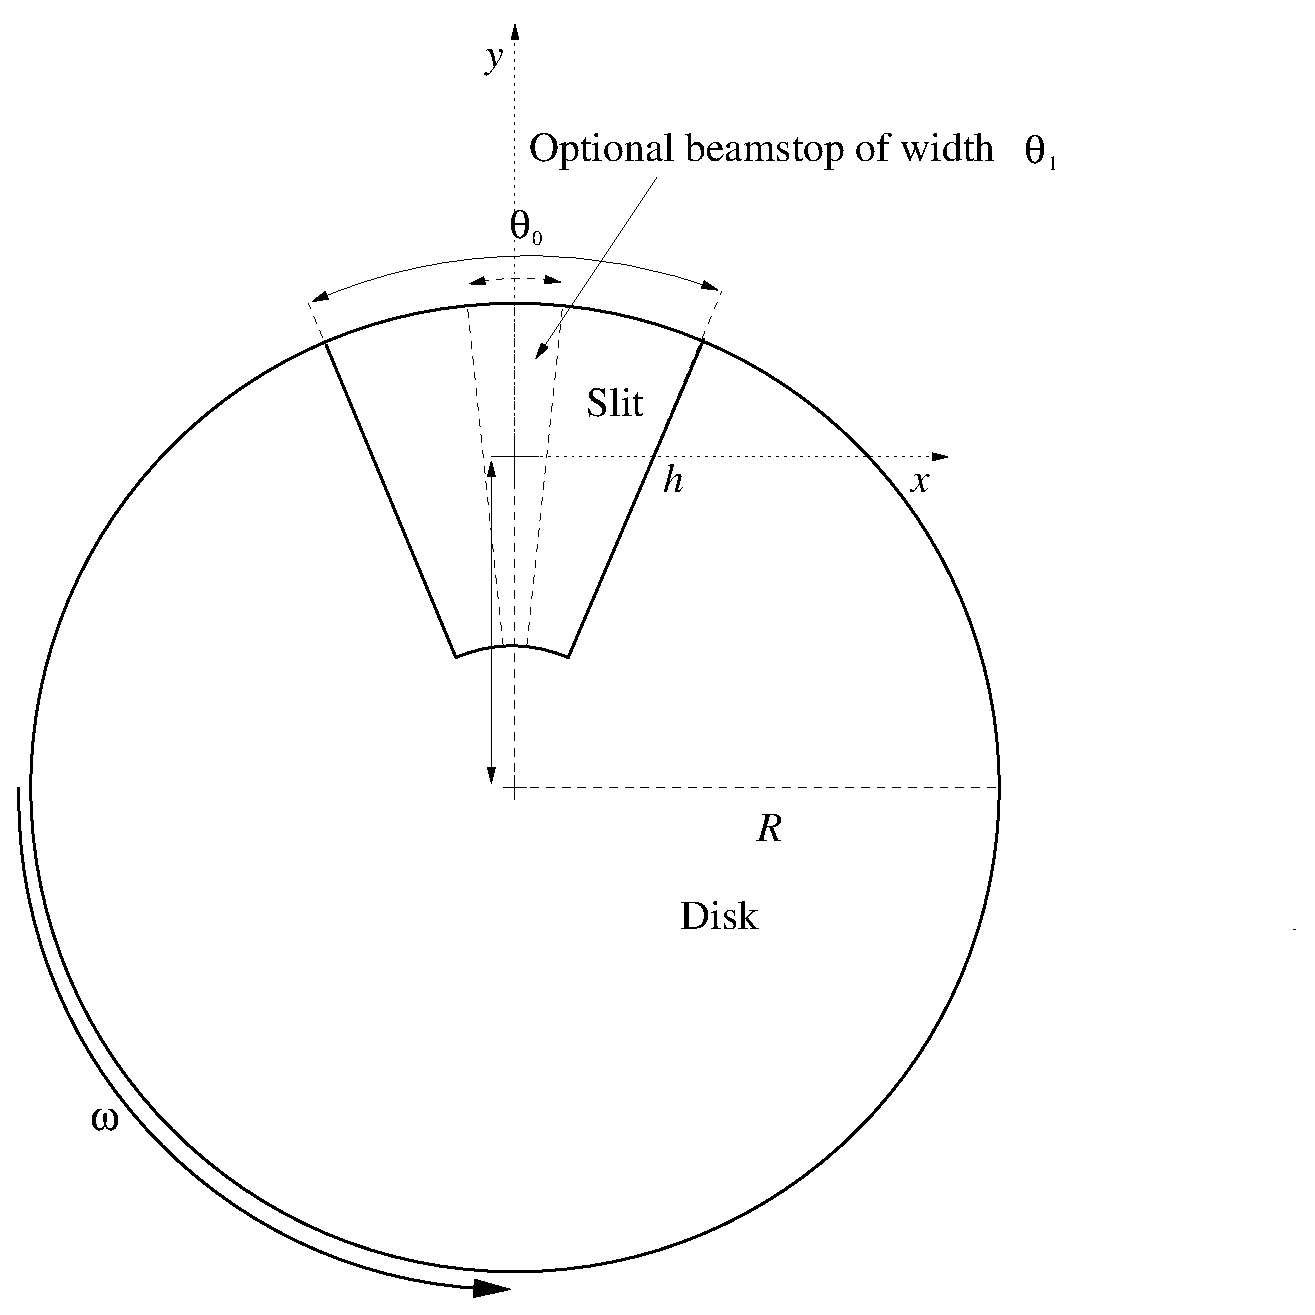
\includegraphics[width=0.8\linewidth]{figures/DiskChopper}
\caption{Sketch of a disc chopper with geometry parameters}
\label{f:chopper1}
\end{figure}


%Using a rectangular shaped beam with nearly the same
%size as the slit, yields an almost triangular shaped
%transmission curve (see figure~\ref{f:chopper2}).
%
%\begin{figure}[ht]
%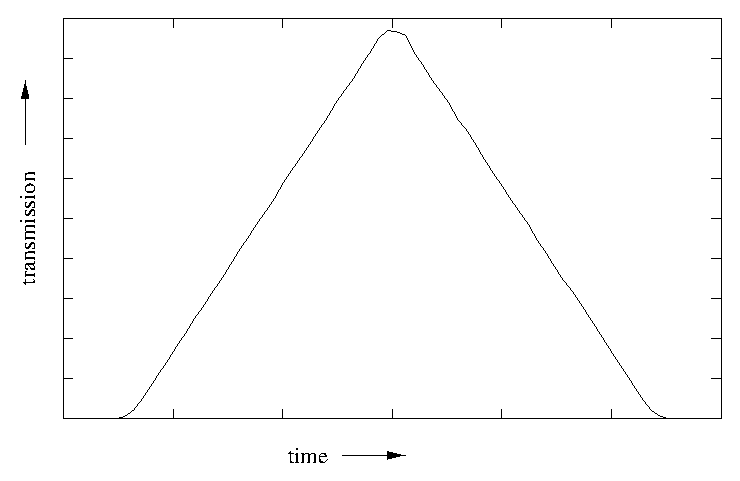
\includegraphics[width=1.0\linewidth]{figures/tracho}
%\caption{example transmission curve for the disc chopper\label{f:chopper2}}
%\end{figure}

When simulating the chopping of a continuous beam,
most of the neutrons could easily be lost.
To improve efficiency, one can set the flag \verb+IsFirst+, which will
allow every neutron ray to pass the {\bf DiskChopper}, but modify the
time, $t$, to a (random) time at which it is possible to pass.
%This can also be used with TOF-instruments, which often
%define the starting time of the neutrons at
%the position of the first chopper.
Of course, there should be only one ``first chopper'' in
any simulation.
To simulate frame overlap from a ``first chopper'', one can specify
the number of frames to study by the parameter $n_{\rm pulse}$.

For more advanced chopper geometries than those mentioned above, it is
possible to set up a \texttt{GROUP} of choppers:

\begin{lstlisting}
COMPONENT Chop1 = DiskChopper(omega=2500, R=0.3, h=0.2, theta_0=20, n=1)
AT (0, 0, 1.1) RELATIVE Source
GROUP Choppers

COMPONENT Chop2 = DiskChopper(omega=2500, R=0.3, h=0.2, theta_0=20, n=1,
                              phi_0=40)
AT (0, 0, 1.1) RELATIVE Source
GROUP Choppers
\end{lstlisting}

The result of such a {\bf DiskChopper} \texttt{GROUP}ing can be seen in
figure \ref{f:chopper2}

\begin{figure}[ht]
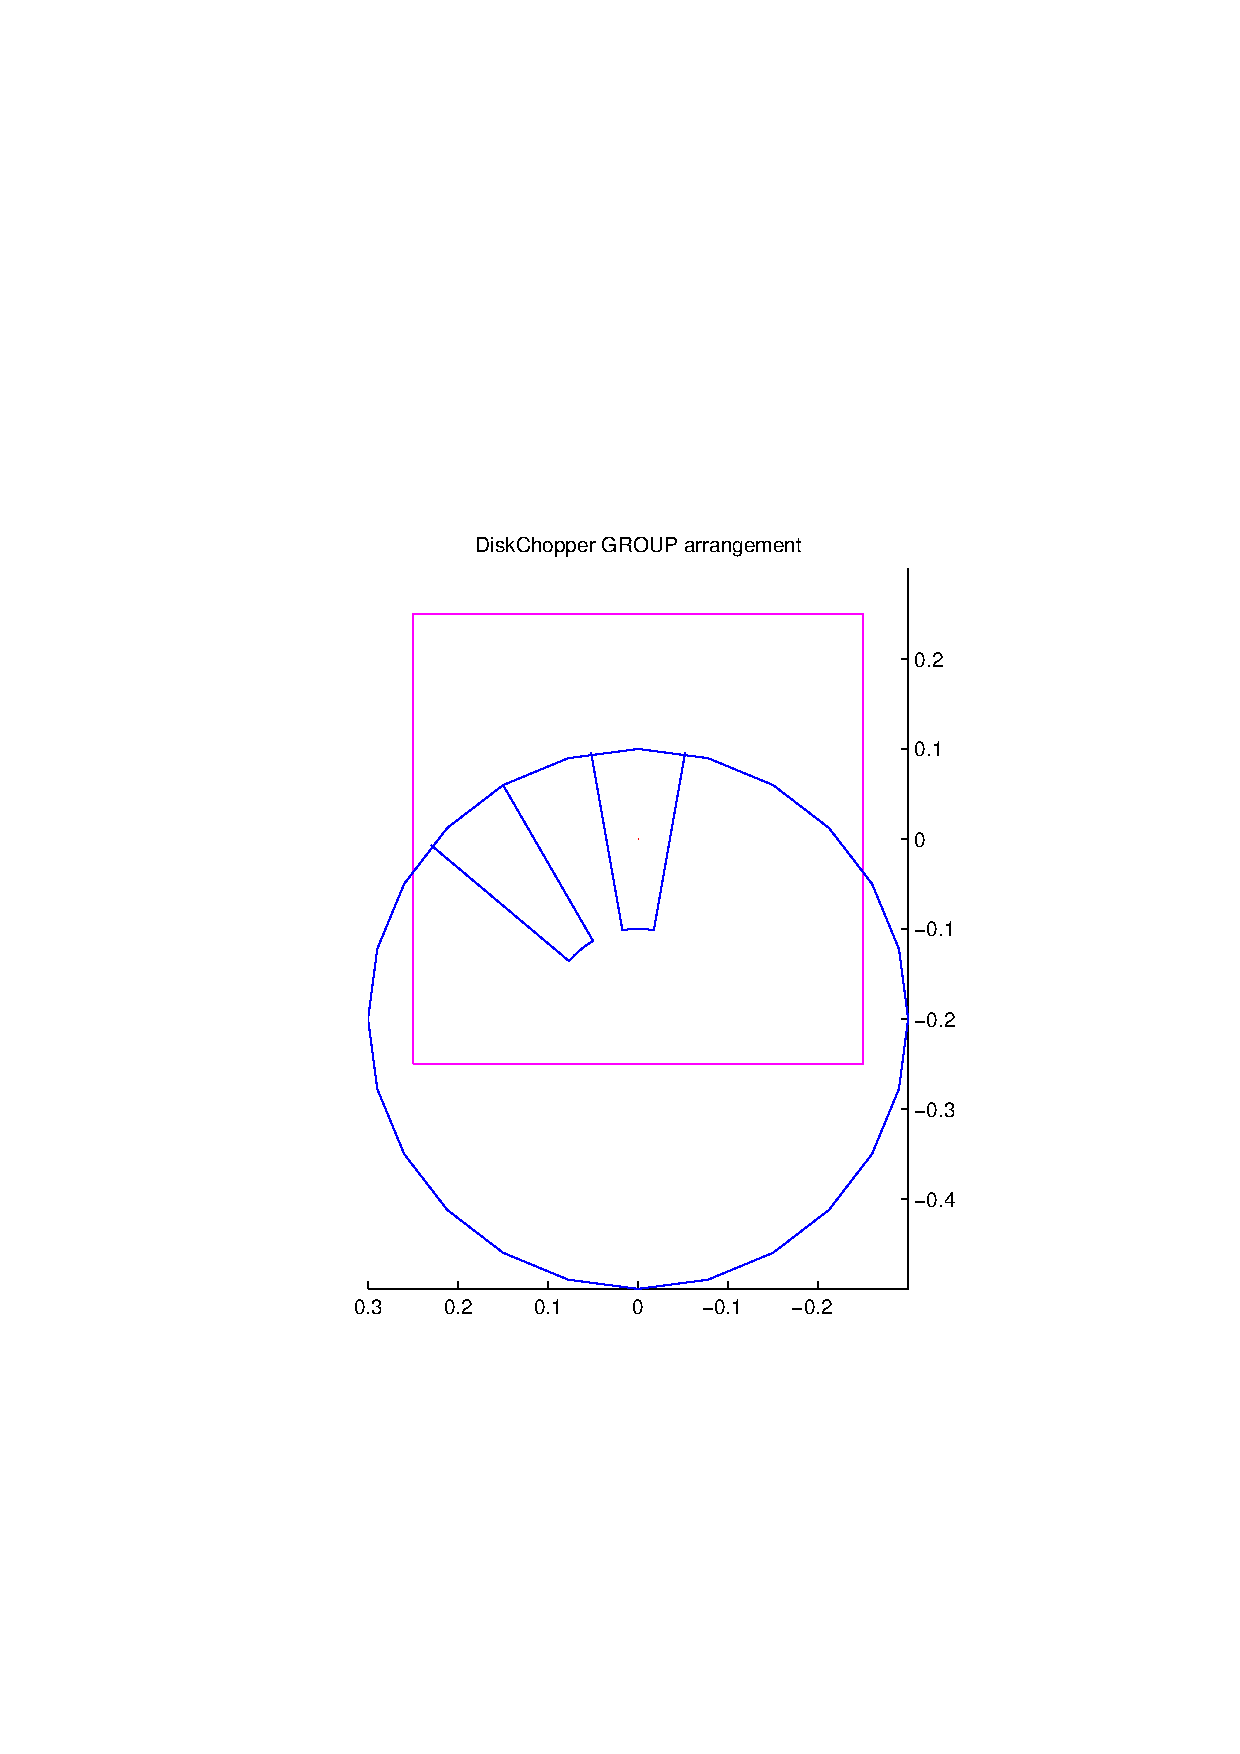
\includegraphics[width=0.4\linewidth]{figures/DiskChopperGroup}
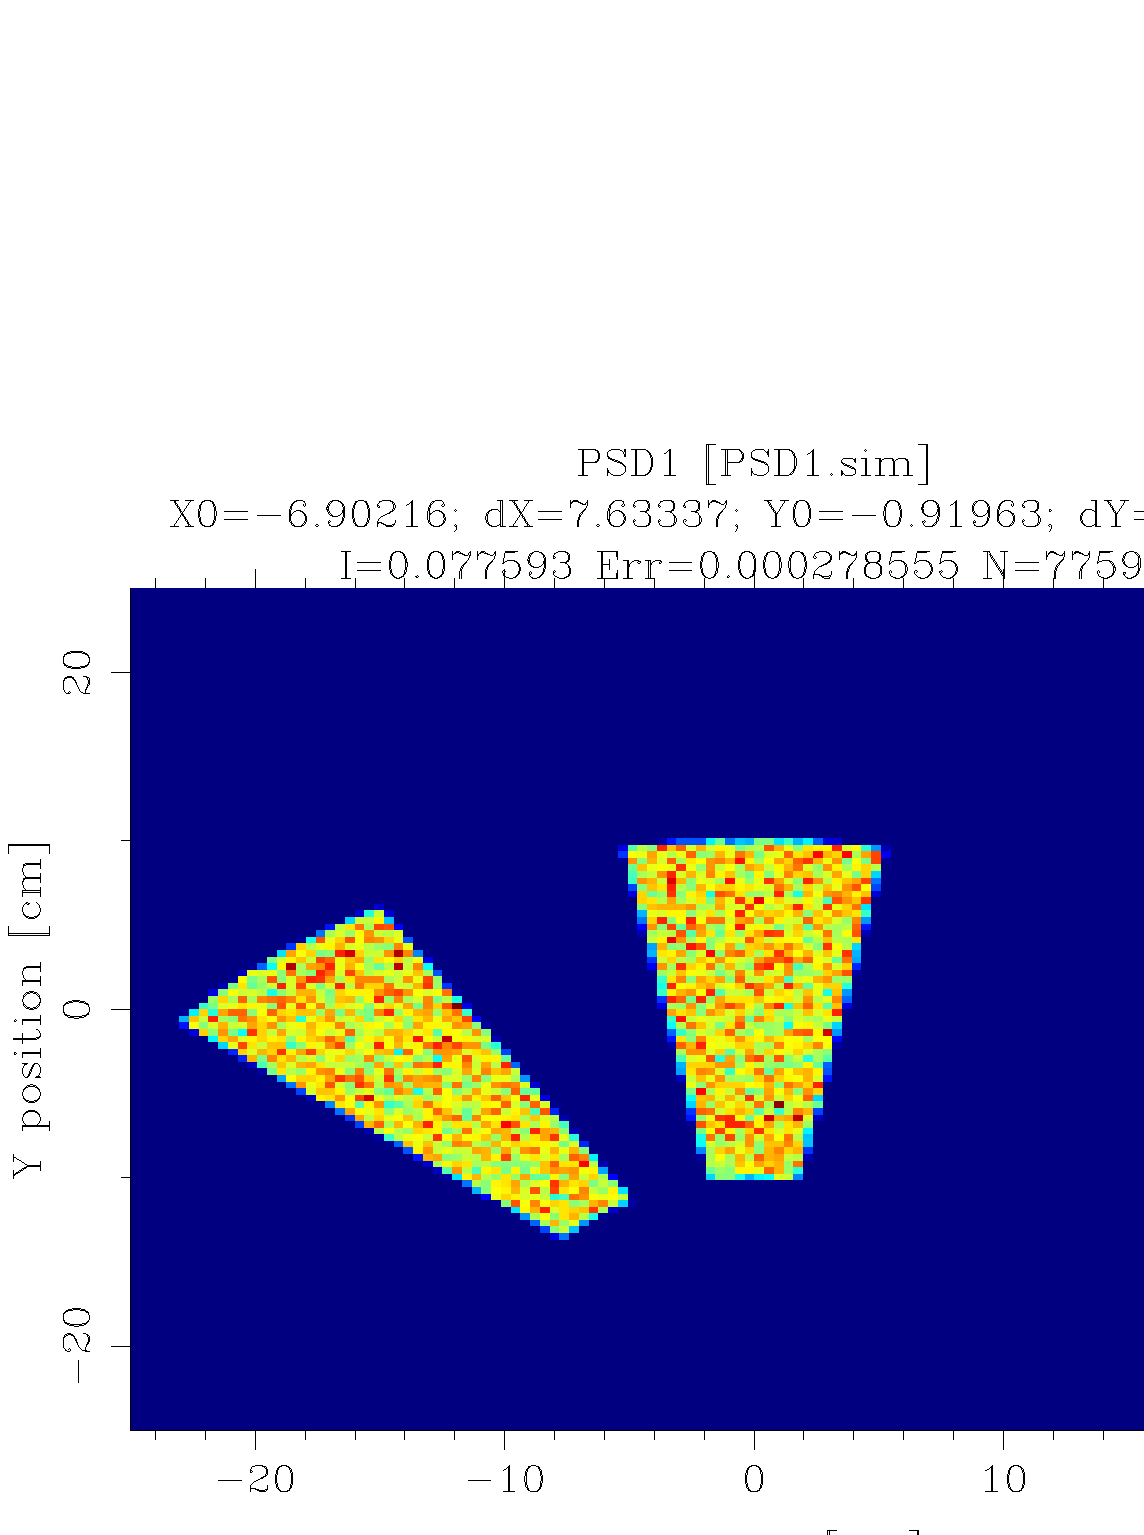
\includegraphics[width=0.4\linewidth]{figures/DiskChopperPSD}
\caption{\texttt{mcdisplay} rendering and monitor output from a DiskChopper \texttt{GROUP}}
\label{f:chopper2}
\end{figure}


\newpage
\section{FermiChopper: The Fermi-chopper}

%\component{FermiChopper}{M. Poehlmann, C. Carbogno, H. Schober,
%E. Farhi}{$R,y_{min} y_{max},
%\nu,w,length$,Nslit,phase}{$m,Q_c,R_0,\alpha,
%W$,curvature,zero\_time}{validated}
\mcdoccomp{optics/FermiChopper.parms}   
\index{Optics!Fermi Chopper|textbf}

\begin{figure}
\begin{center}
\begin{tabular}{cc}
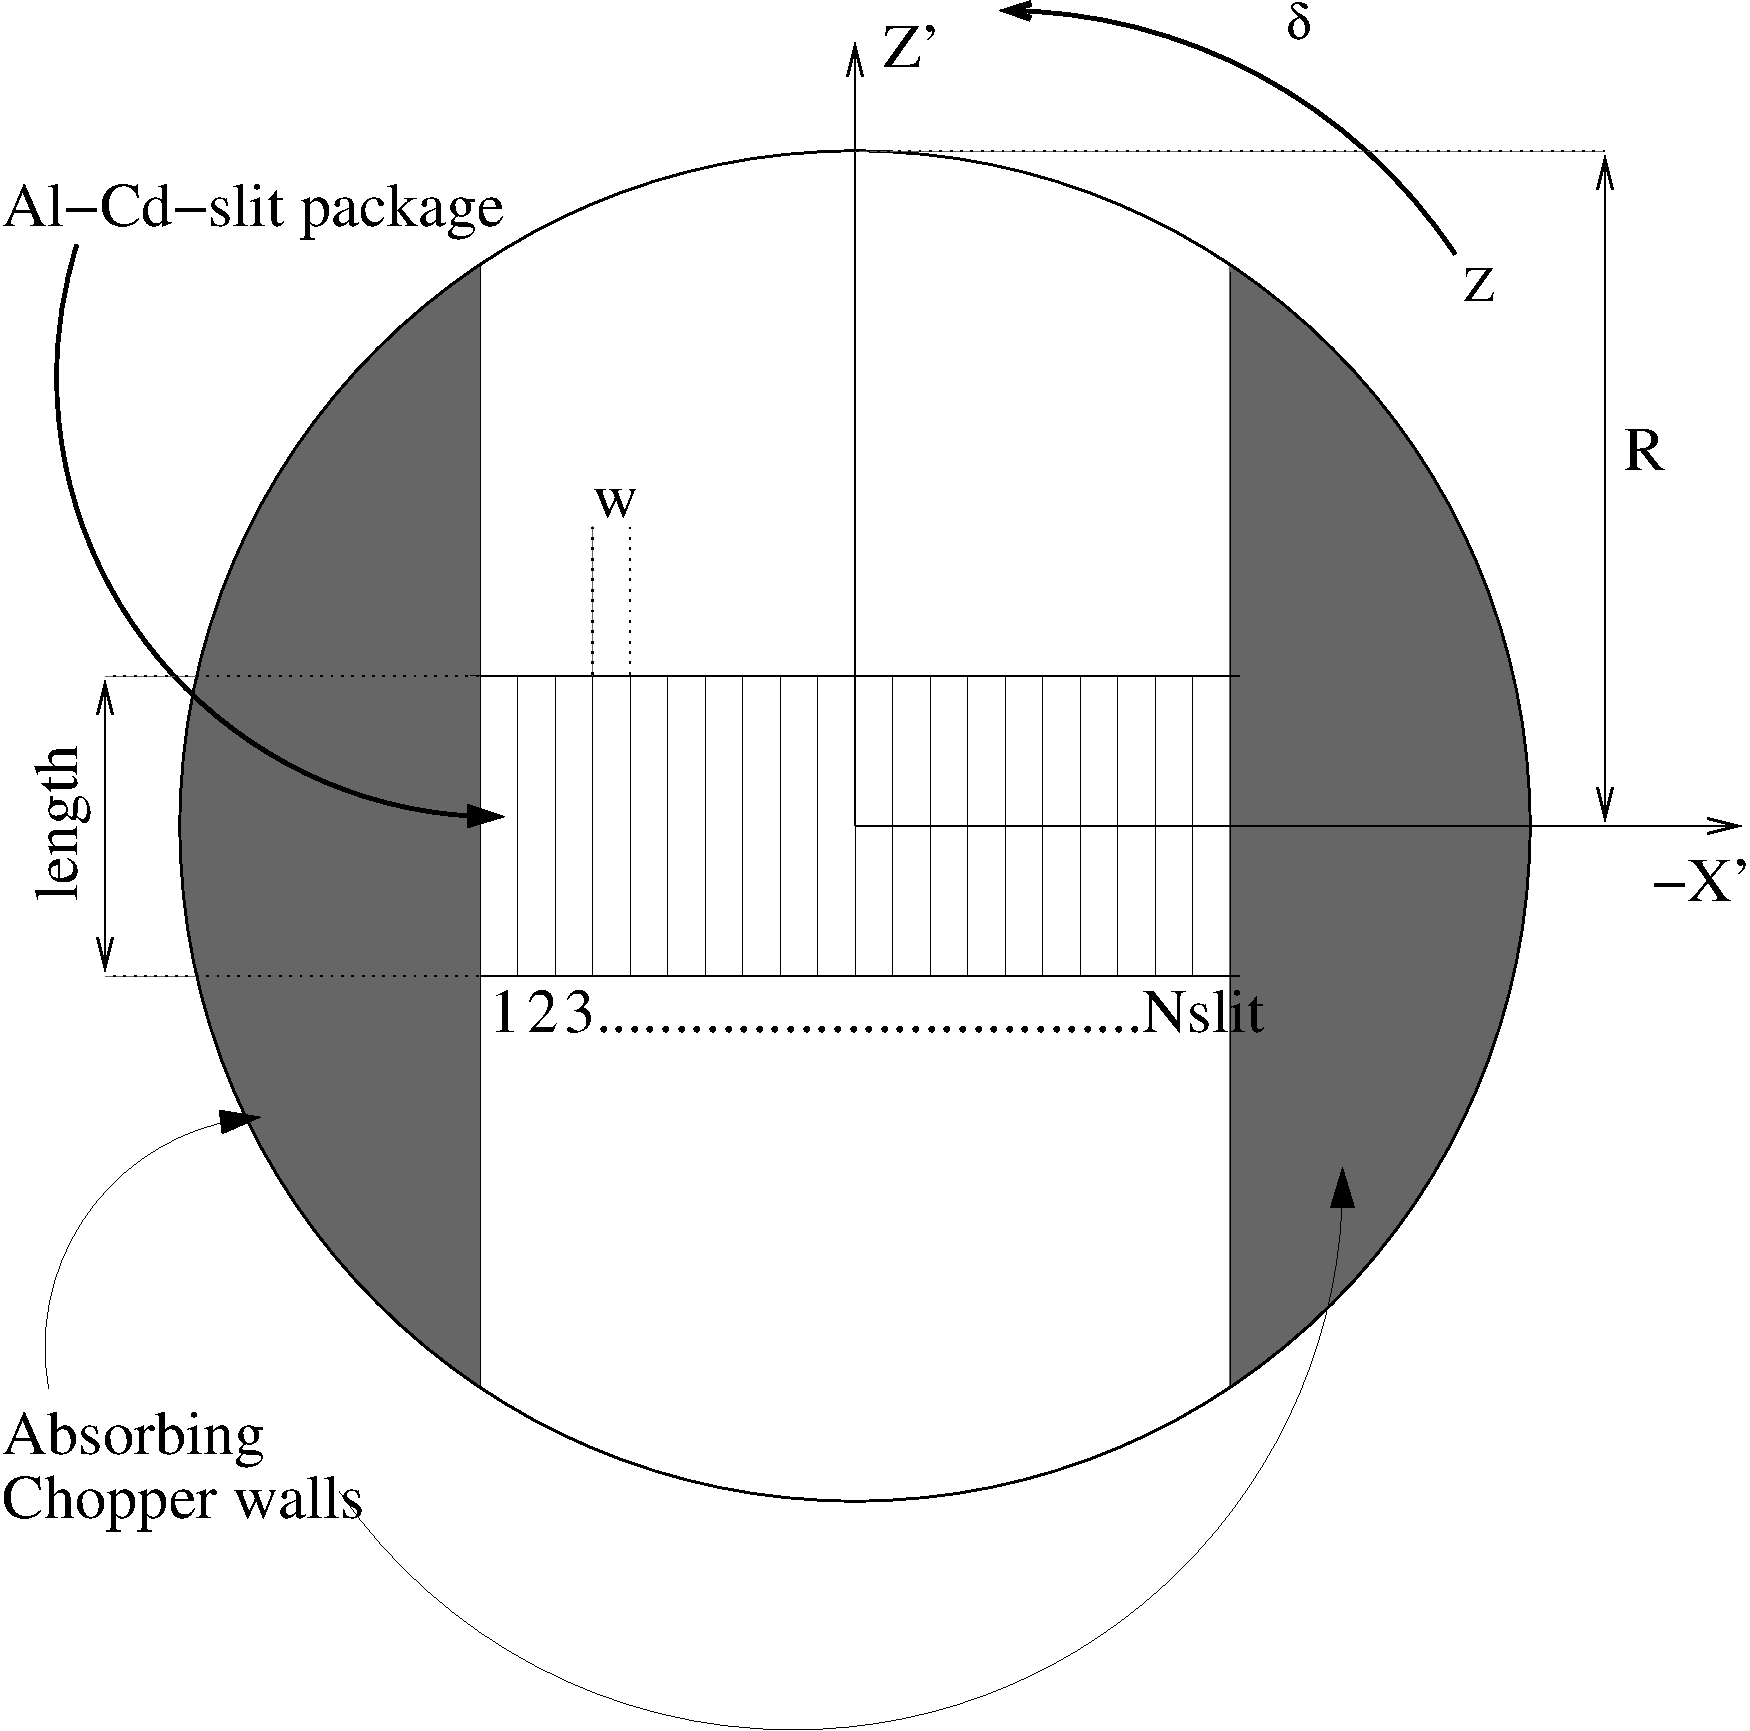
\includegraphics[height=7cm]{./figures/FCChoppergeo}
&
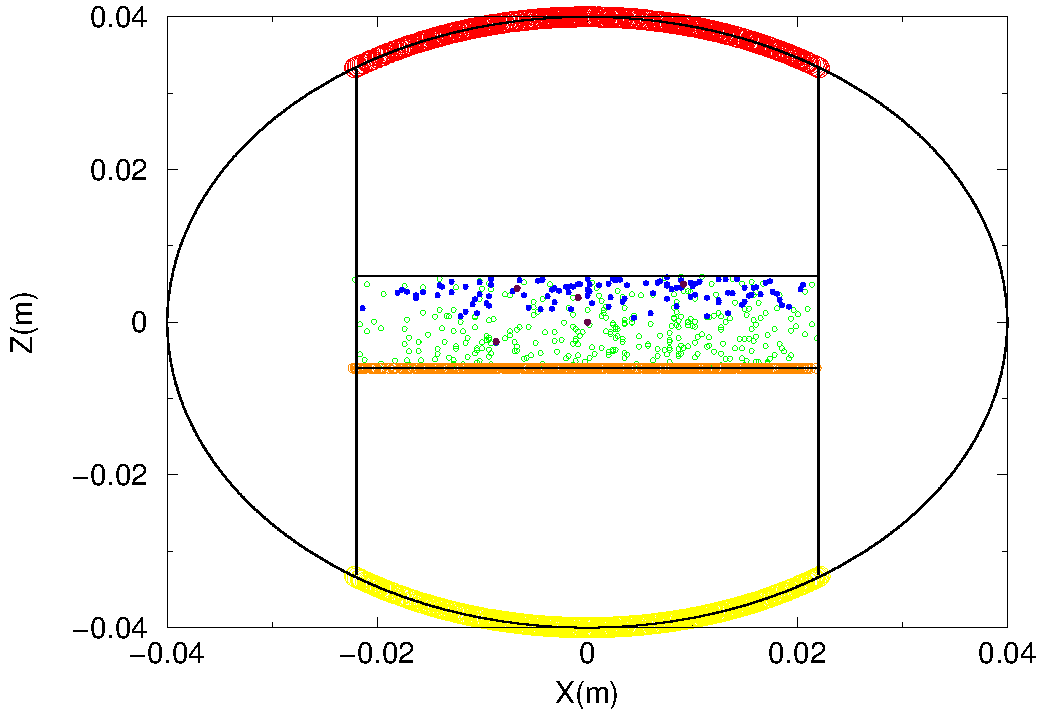
\includegraphics[height=5cm,width=5.3cm]{./figures/FCOverview}
\end{tabular}
\end{center}
\caption{Geometry of the Fermi-chopper (left) and Neutrons in the chopper (right).}
\label{fig:Overview}
\end{figure}

\subsection{The chopper geometry and parameters}
\label{ssec:chopper}

The Fermi chopper is a rotating vertical cylinder containing a set of collimating slits (\emph{slit package}). Main geometry parameters are the radius $R$, minimum and maximum height $y_{min}$ and $y_{max}$ (see Fig. \ref{fig:Overview}).
In this implementation, the slits are by default straight, but may be coated with super-mirror, and curved. Main parameters for the slits are the number of slits $Nslit$, the length $length$ and width $w$ of each slit, the width of the separating Cd-blades is neglected. The slit walls reflectivity is modelled just like in guide components by the $m$-value ($m > 1$ for super mirrors), the critical scattering vector $Q_c$, the slope of reflectivity $\alpha$, the low-angle reflectivity $R_0$ and the width of supermirror cut-off $W$. For $m=0$ the blades are completly absorbing. The AT position of the component is its center.

The angular speed of the chopper is $\omega = 2\pi \nu$, where $\nu$ is the rotation frequency. The angle $phase$ for which the chopper is in the 'open' state for most of the neutrons coming in (z' axis of the rotating frame parallel to the z axis of the static frame) is also an input parameter. The time window may optionally be shifted to zero when setting the \verb+zero_time=1+ option. A phase guess value may be set automatically using the \verb+zero_time=2+ option.

The curvature of the slit channels is specified with the {\it curvature} parameter. Positive sign indicates that the deviation 'bump' due to curvature is in the $x'$ positive side, and the center of curvature is in the $x'$ negative side. The optimal radius of curvature $R$ is related to frequency $\nu$ and neutron velocity $v$ with: $v=4 \pi R \nu$.

The component was validated extensively by K.\ Lieutenant. As an alternative, one may use the {\bf Vitess\_ChopperFermi} component (eventhough slower and without super-mirror support) or the {\bf FermiChopper\_ILL} contributed component. The Guide\_gravity component has also a rotating mode, using an approximation of a Fermi Chopper.

\begin{table}
  \begin{center}
  {\let\my=\\
    \begin{tabular}{|lr|p{0.6\textwidth}|}
    \hline
Parameter & unit & meaning \\
    \hline
radius & [m] & chopper cylinder radius \\
ymin   & [m] &   lower y bound of cylinder \\
ymax   & [m] &   upper y bound of cylinder \\
Nslit  & [1] &   number of chopper slits \\
length & [m] &   channel length of the Fermi chopper \\
w      & [m] &   width of one chopper slit. May also be specified as \emph{width}=w*Nslit for total width of slit package. \\
nu & [Hz] &  chopper frequency \\
phase     & [deg] &   chopper phase at t=0 \\
zero\_time & [1] & shit time window around 0 if true \\
curvature & [m$^{-1}$] & Curvature of slits (1/radius of curvature) \\
    \hline
m     & [1] & \\
alpha & [\AA] & \\
Qc    & [\AA$^{-1}$] & slit coating parameters. See section \ref{ss:mirrorreflect} \\
W     & [\AA$^{-1}$] & \\
R0    & [1] & \\
    \hline
    \end{tabular}
    \caption{FermiChopper component parameters}
    \label{t:fc-param}
  }
  \end{center}
\end{table}


\subsection{Propagation in the Fermi-chopper}

As can be seen in figure \ref{fig:Overview}, neutrons first propagate onto the cylinder surface of the chopper (yellow curve). Then the program checks the interaction with the entrance of the slit package (orange line) and calculates which slit is hit. If the slit coating is reflecting ($m > 0$), multiple reflections are calculated (green, blue and maroon circles), otherwise the neutrons are absorbed as soon as they interact with the blades. Finally the remaining neutrons propagate to the exit of the chopper (red curve).

The rotation of the chopper is characterized by the angle $\delta$ between the rotating z' and the static z-axis. $\delta(t)$ is defined by:

$$\delta(t) = \widehat{z,z'} = \omega.(t-t_0) = \omega.t+\phi_0$$

where $t$ is the absolute time, $t_0$ is the chopper delay, and $\phi_0$ is the chopper phase. The chopper should better be \emph{time focussing}: slow neutrons should pass before the fast ones, so that they finally hit the detectors at the same time. Therefore the signs of $\omega$ and $\delta$ are very important: For $t>t_0$, $\delta$ is positive and points anti-clockwise.

Since the rotation is applied along the y - axis, we can simplify the problem to two dimensions. The orthogonal transformation matrix $T$ from the static $(zx)$ to the rotating frame $(z'x')$ is:
\begin{equation}
T_{zx \rightarrow z'x'} = \left(
\begin{array}{cc}
\cos(\delta) & \sin (\delta) \\
-\sin(\delta) & \cos(\delta)
\end{array}
\right)
\end{equation}

\begin{figure}
\begin{center}
\begin{tabular}{cc}
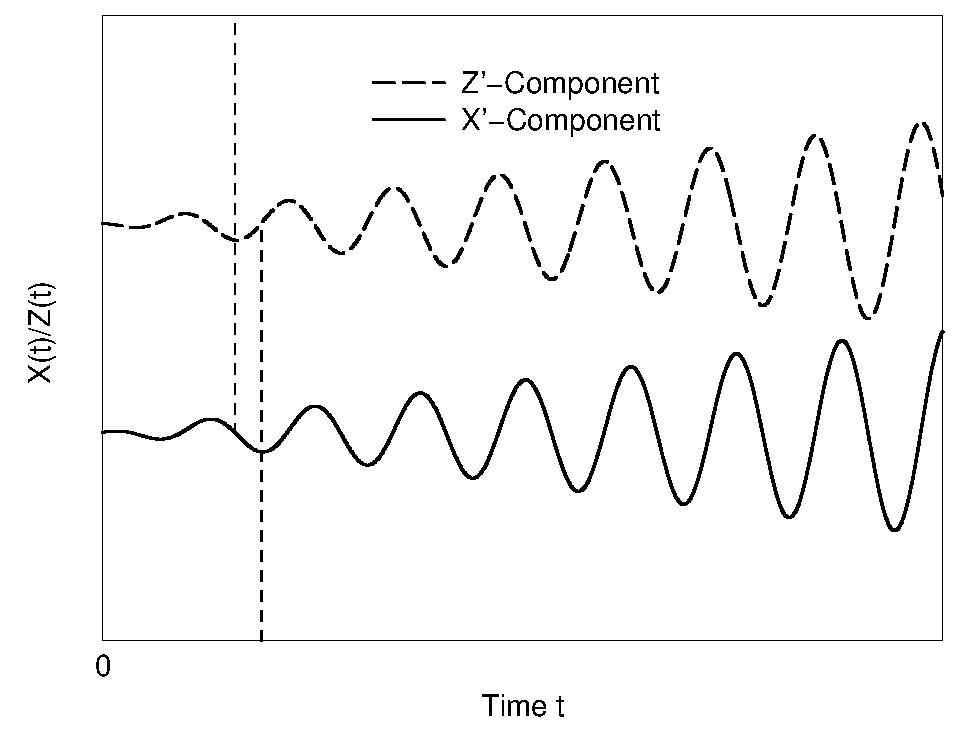
\includegraphics[height=5.5cm]{./figures/XZCoords}
&
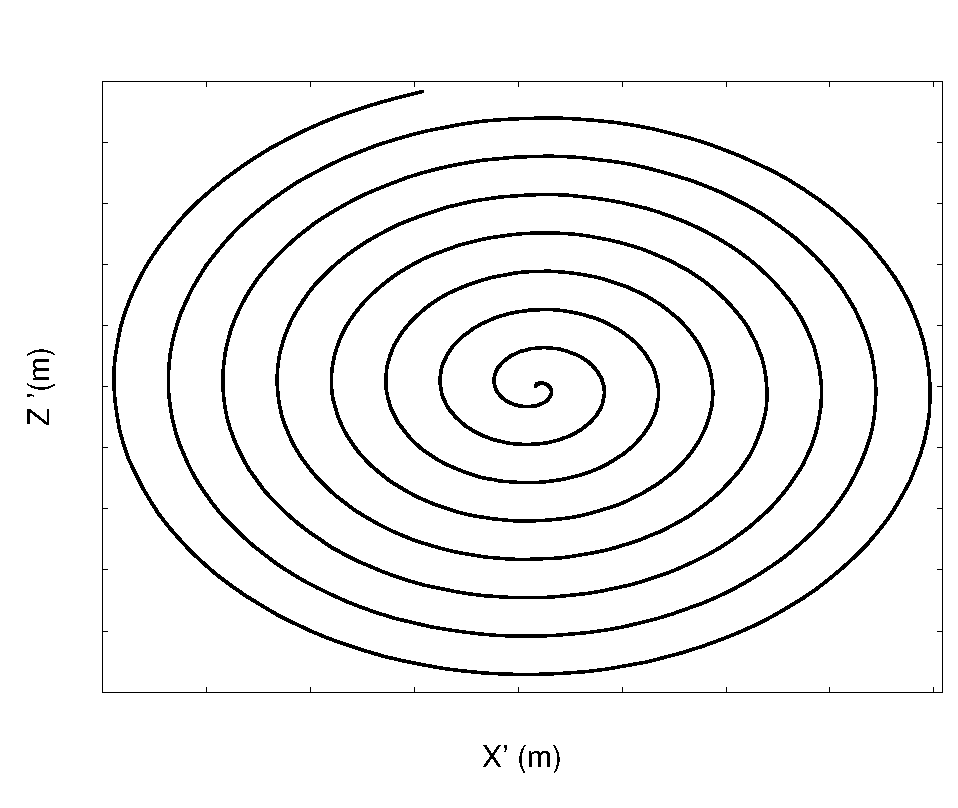
\includegraphics[height=6.5cm,width=5.5cm]{./figures/XZplain}
\end{tabular}
\end{center}
\caption{The x' and z' component as a function of time in the rotating frame (left). A typical neutron trajectory in the rotating frame (right).}
\label{fig:Component}
\end{figure}

Together with the equation for a non-accelerated, linear propagation $\vec{r} = \vec{r_0}+\vec{v}t$ the orthogonal transformation produces a curve in the Z'-X'-plane known as \emph{archidemic spiral}, as can be seen in figure \ref{fig:Component}. The two vector components $s(t) = (z',x')$ follow the equation:
\begin{equation}
s(t) = \left(
\begin{array}{c}
z' \\
x'
\end{array}
\right) = T.\left(
\begin{array}{c}
z(t) \\
x(t)
\end{array}
\right) = \left(
\begin{array}{c}
(z_0+v_z.t)cos(\delta(t)) + (x_0+v_x.t)sin(\delta(t)) \\
-(z_0+v_z.t)sin(\delta(t)) + (x_0+v_x.t)cos(\delta(t))
\end{array}
\right).
\label{eq:Txz}
\end{equation}
For a fixed chopper rotation speed, the neutron trajectory tends to strech from a spiral curve for slow neutrons to a straight line for fast neutrons. For real Fermi chopper settings $\nu$ (about 100 Hz on IN6 at the ILL), neutron trajectories are found to be nearly straight for 1000 m/s neutron velocities \cite{blanc83}.

The basis of the algorithm is to find the intersections of these spiral trajectories with the chopper outer cylinder and then the slit package, in the rotating frame.

For this purpose, the \emph{Ridders's} root finding method was implemented \cite{NumRecip} in order to solve
\begin{equation}
x'(t) = d {\rm\ or\ } z'(t) = d
\label{eq:Ridder}
\end{equation}
This method provides faster and more accurate intersection determination than other common algorithms. E.g. the secant method fails more often and may give wrong results (outside chopper) whereas the bisection method (a.k.a Picard dichotomy) is slightly slower.

\subsubsection{Standard slit packages (non super-mirror)}

\begin{figure}
\begin{center}
\begin{tabular}{cc}
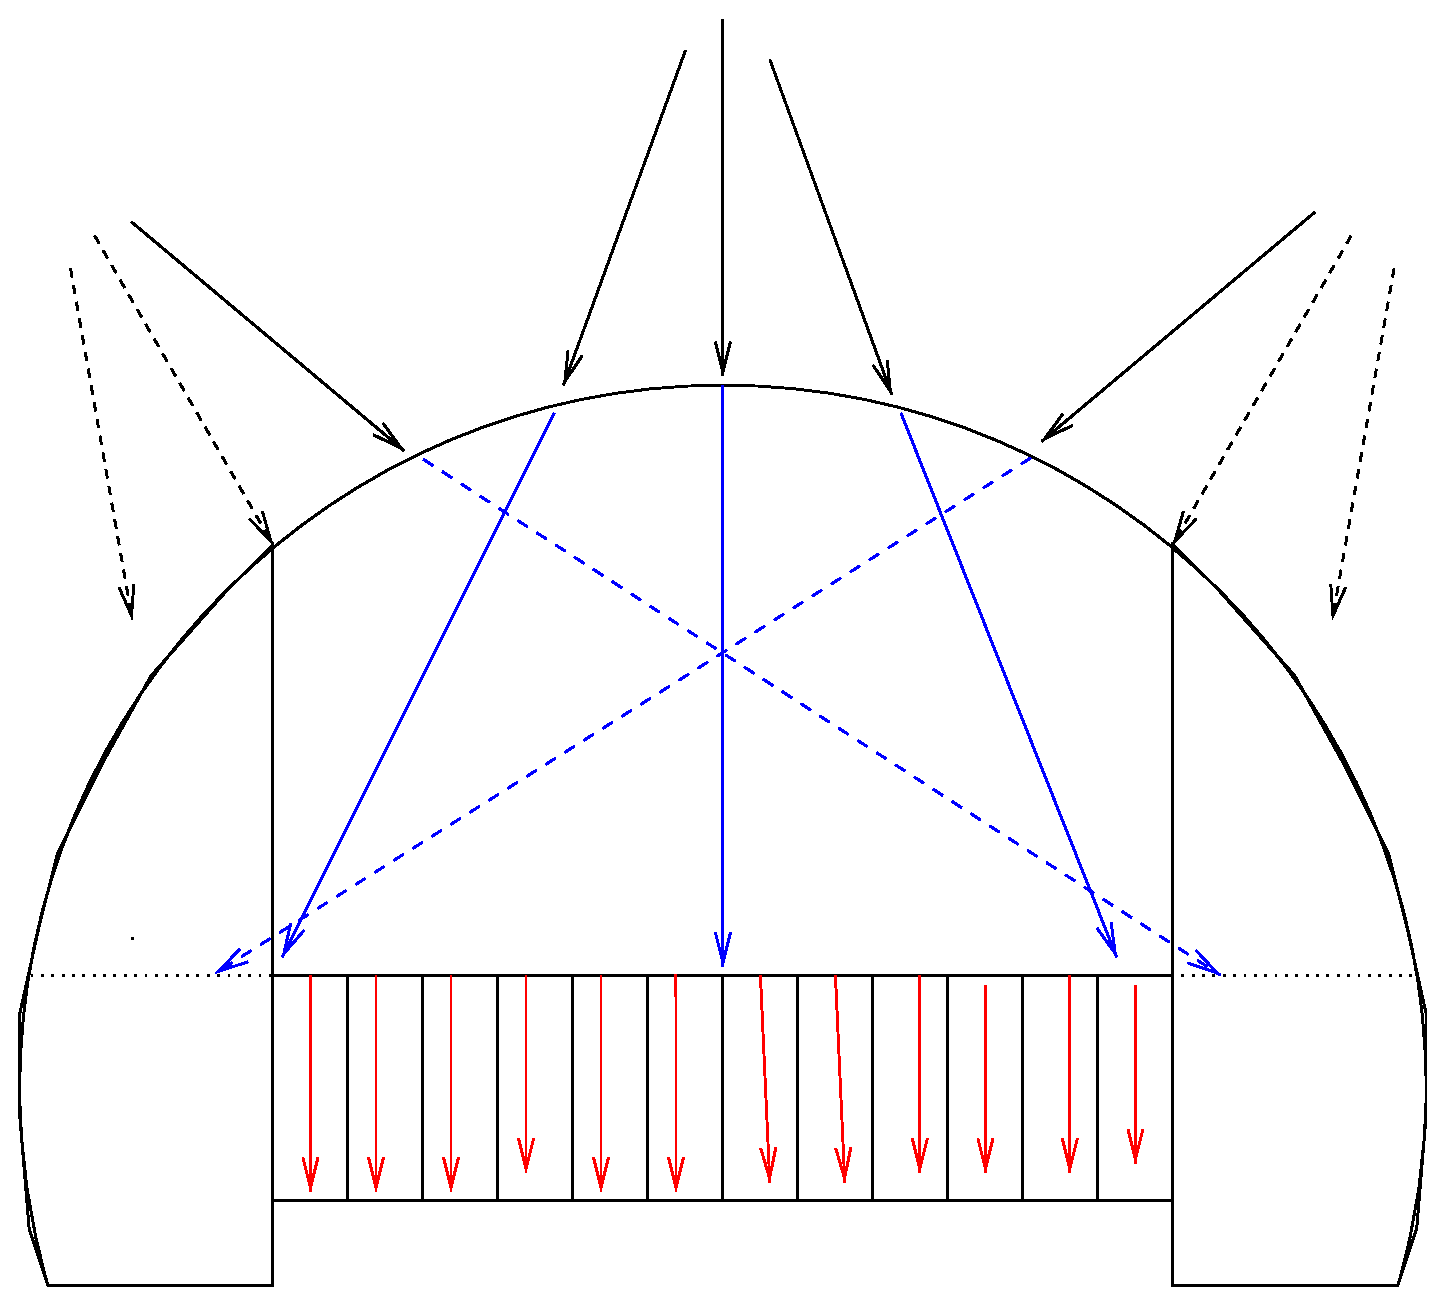
\includegraphics[height=5cm]{./figures/FCAlgo}
&
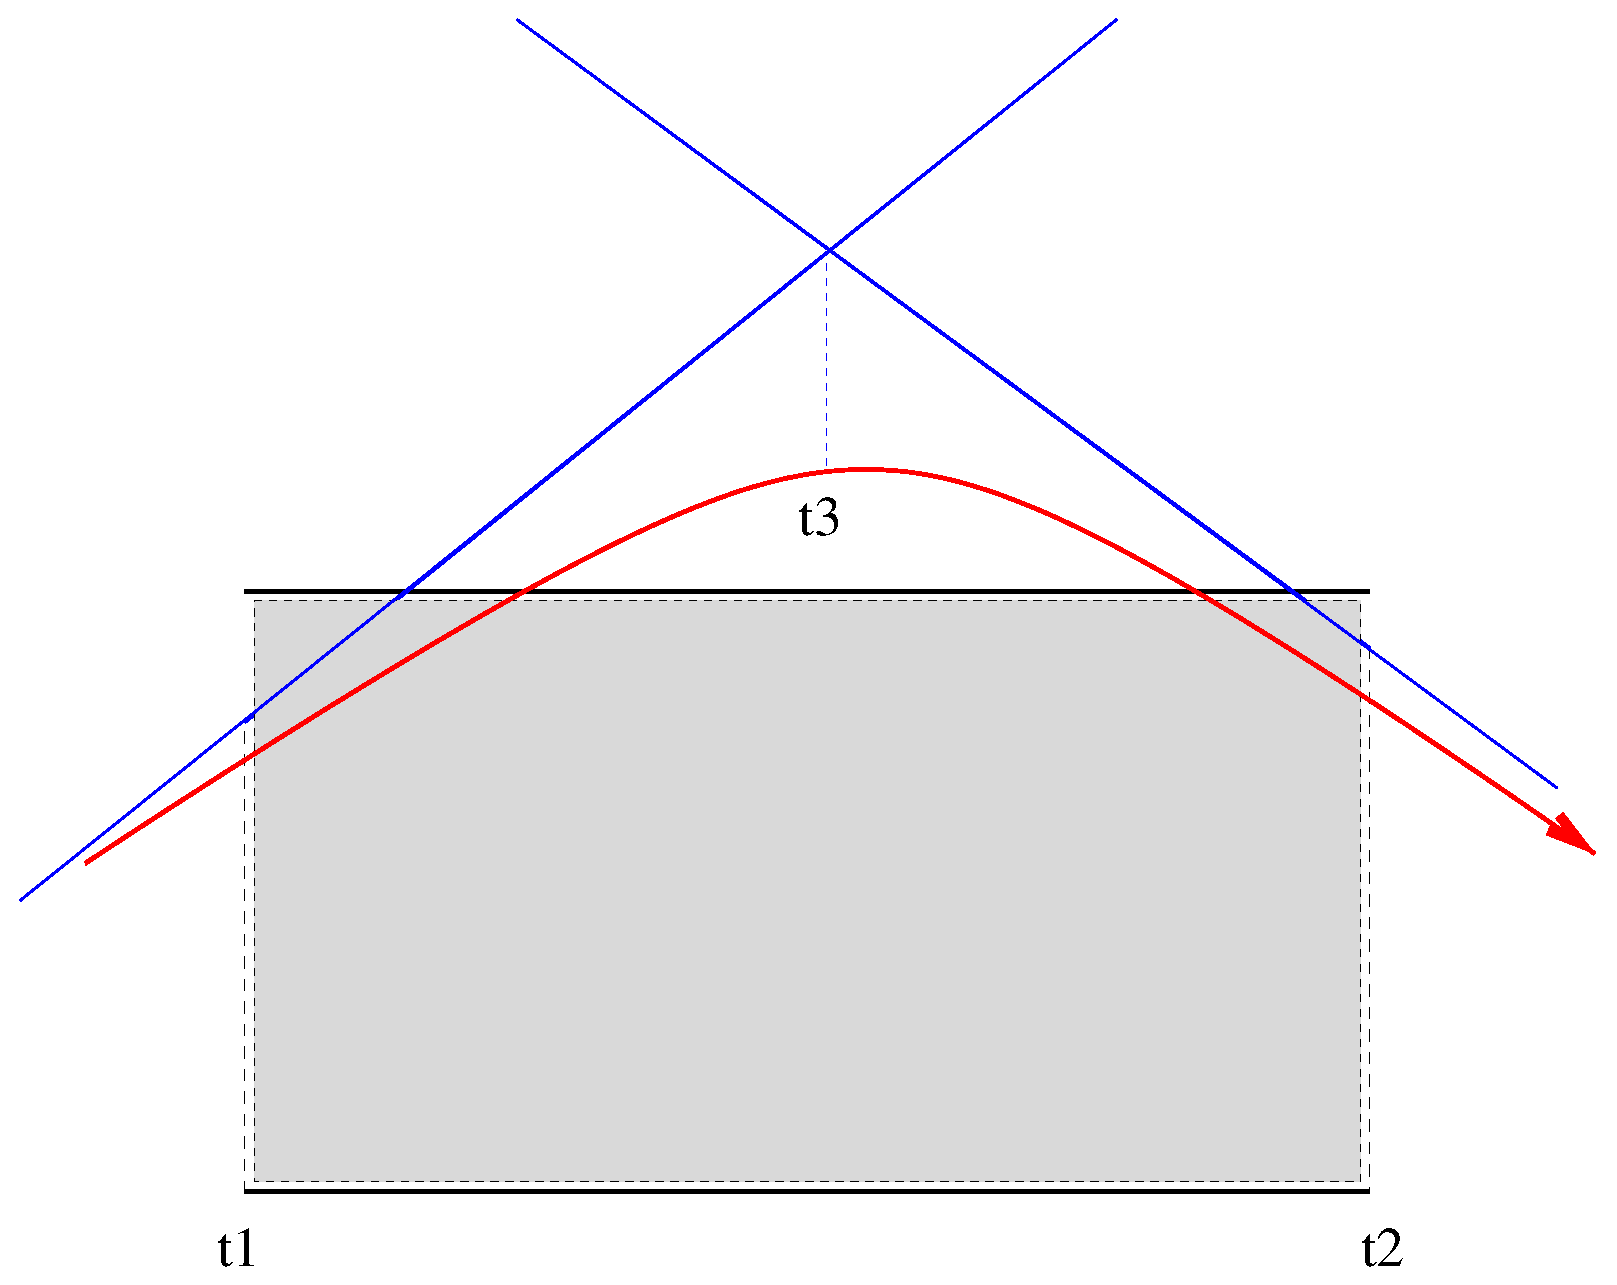
\includegraphics[height=5cm]{./figures/FCtangents}
\end{tabular}
\end{center}
\caption{The different steps in the algorithm (left). A neutron trajectory in a slit (right)}
\label{fig:TOFalg}
\end{figure}

The neutrons are first propagated to the outer chopper cylinder and their coordinates are transformed into the rotating frame using $T$. Neutrons outside the slit channel (chopper opening), or hitting the top and bottom caps are absorbed (yellow dots in Fig. \ref{fig:Overview}). The side from which the neutron approaches the chopper is known (positive or negative z'-axis of the rotating frame) so that the calculation of the time of interaction with the slit package entrance $t_1$ is performed solving $z' = \pm \frac{\rm length}{2}$ in Eq. (\ref{eq:Txz}). Using the result of the numerical algorithms the neutron propagates to the entrance of the slit package (orange circles in Fig. \ref{fig:Overview}). Neutrons getting aside the slit package entrance are absorbed. Additionally, the slit package exit time $t_2$ is estimated the same way with $z' = \mp \frac{\rm length}{2}$, in order to evaluate the whole time-of-flight in the chopper. The index of the slit which was hit is also computed, as we know the $x'$ coordinate in the rotating frame at the slit entrance.

Differentiating Eq. (\ref{eq:Txz}) for $x$ coordinate
\begin{equation}
\dot{x'}(t) = v_x'(t) = [v_x-\omega.(z+v_z.t)]\cos(\omega(t-t_0)) - [v_z+\omega.(x+v_x.t)]\sin(\omega(t-t_0))
\end{equation}
we may estimate the tangents to the spiral neutron trajectory in the rotating frame at times $t_1$ and $t_2$. The intersection of these two lines gives an intermediate time $t_3$.

If the neutron remains in the same slit at this point, then there is no intersection with the slit walls (direct flight), and the neutron may be propagated to the slit output, and then to the cylinder output. A last check is made for the neutron to pass the chopper aperture in the cylinder.

If the neutron changes of slit channel at this point, we may determine the intersection time of the neutron trajectory within $[ t_1, t_3 ]$ or $[ t_3, t_2 ]$, as seen in Fig. \ref{fig:TOFalg}. If walls are not reflecting, we just absorb neutrons here.

\subsubsection{The reflections (super-mirror slits)}

If slit walls are reflecting, neutron is first propagated to the slit separating surface. Then the velocity in the rotating frame is computed using Eq. (\ref{eq:Txz}). Perpendicular velocity $v_x'$ is reverted for reflection, and inverse $T$ transformation is performed. Reflected intensity is computed the same way as for the guide component (see section \ref{s:mirror}). The remaining time $t_2$ to the slit output is estimated and the tangent intersection process is iterated, until neutron exits. Remember that super mirror $m < 1$ parameters behave like $m=1$ materials (see section \ref{ss:mirrorreflect}). Selecting $m=0$ sets the blabes absorbing.

The propagation is finalized when determining the intersection of the neutron trajectory with the outer surface of the chopper cylinder. The neutron must then pass its aperture, else it is absorbed.

\subsubsection{Curved slit packages}

The effect of curvature can significantly improve the flux and energy resolution shape.

As all $(zx)$ cordinates are transformed into $(z'x')$, the most efficient way to take into account the curvature is to include it in the transformation Eq. (\ref{eq:Txz}) by 'morphing' the curved rotating real space to a straight still frame. We use parabolic curvature for slits. Then instead of solving
\begin{equation}x'(t) = d - \Delta_{x'}(z') {\rm\ where\ } \Delta_{x'}(z')=R_{slit}.(1-\sqrt{1-(z'/R_{slit})^2})
\end{equation}
with $\Delta$ being the gap between the straight tangent line at the slit center and the real slit shape, we perform the additional transformation
\begin{equation}
x' \rightarrow x' + \Delta_{x'}(z')
\end{equation}
The additional transformation counter-balances the real curvature so that the rest of the algorithm is written as if slits were straight.
This applies to all computations in the rotating frame, and thus as well to reflections on super mirror coatings.



% Emacs settings: -*-mode: latex; TeX-master: "manual.tex"; -*-

\section{Vitess\_ChopperFermi: The Fermi Chopper from Vitess}
\label{s:vit_fc}
\index{Optics!Fermi Chopper}

\component{Vitess\_ChopperFermi}{Geza Zsigmond}{GeomOption, $N_{\rm chan}$, $f$, $h$, $w_{\rm tot}$, $l$, $r_{\rm curv}$, $d$, $\phi$, $w_{\rm wall}$, GeomFile}{zerotime, $N_{\rm gates}$}{validated}


The component {\bf Vitess\_ChopperFermi} simulates a Fermi chopper with absorbing walls.
The shape of the channels can be straight, curved with circular, or curved with ideal
(i.e. close to a parabolic) shape.
This is determined by the parameter 'GeomOption'. In the option 'straight Fermi
chopper', the very fast neutrons are transmitted with only a time modulation and lower
speed neutrons are modulated both in time of flight and wavelength.
If the channels are curved, the highest transmission occurs for a wavelength

\begin{equation}
\lambda_{\rm opt} = \frac{3956 {\rm [m\AA/s]}}{2 \omega r_{\rm curv}}
\end{equation}

with

\begin{equation}
\omega = 2 \pi f
\end{equation}

The optimal shape is calculated in an exact way and is close to parabolic; in this
case, transmission is as high for the optimal wavelength as in the case of a straight
Fermi chopper for the limit $\lambda \rightarrow 0$.
In the more realistic case of circular shapes channels, the transmission is slightly
lower. In general, neutrons are transmitted through a curved Fermi chopper with a time
AND wavelength modulation .

The rotation axis is vertical (y-axis), i.e. the path length through the channels is
given by the length $l$ along the z-axis. The inital orientation is given by the phase
$\phi$ of the chopper - $\phi$ = 0 means transmission orientation.

Geometry for {\bf straight} and {\bf circular} channels:
The geometry of the chopper consists of a rectangular shaped object with a channel
system. In transmission position, there are $N_{\rm gates}$ slits of width $w_{\rm slit}$
each along the x-axis, separated by absorbing walls of thickness $w_{\rm wall}$
(see figure~\ref{f:vit_fc1}). The total width $w_{\rm tot}$ is given by

\begin{equation}
w_{\rm tot} = N_{\rm gates} w_{\rm slit} + (N_{\rm gates}+1) w_{\rm wall}
\end{equation}

The rectangular channel system is surrounded by a so-called shadowing cylinder; it is a
part of a cylinder with vertical symmetry axis and diameter

\begin{equation}
d \geq \sqrt{l^2 + w_{\rm tot}^2}
\end{equation}

It serves to prevent transmission of neutrons which do not fly through the channels;
but it also reduces the transmission, because the cylinder removes neutrons
in front of the channel entrance or behind the channel exit (see figure~\ref{f:vit_fc1}).

\begin{figure}[ht]
\begin{center}
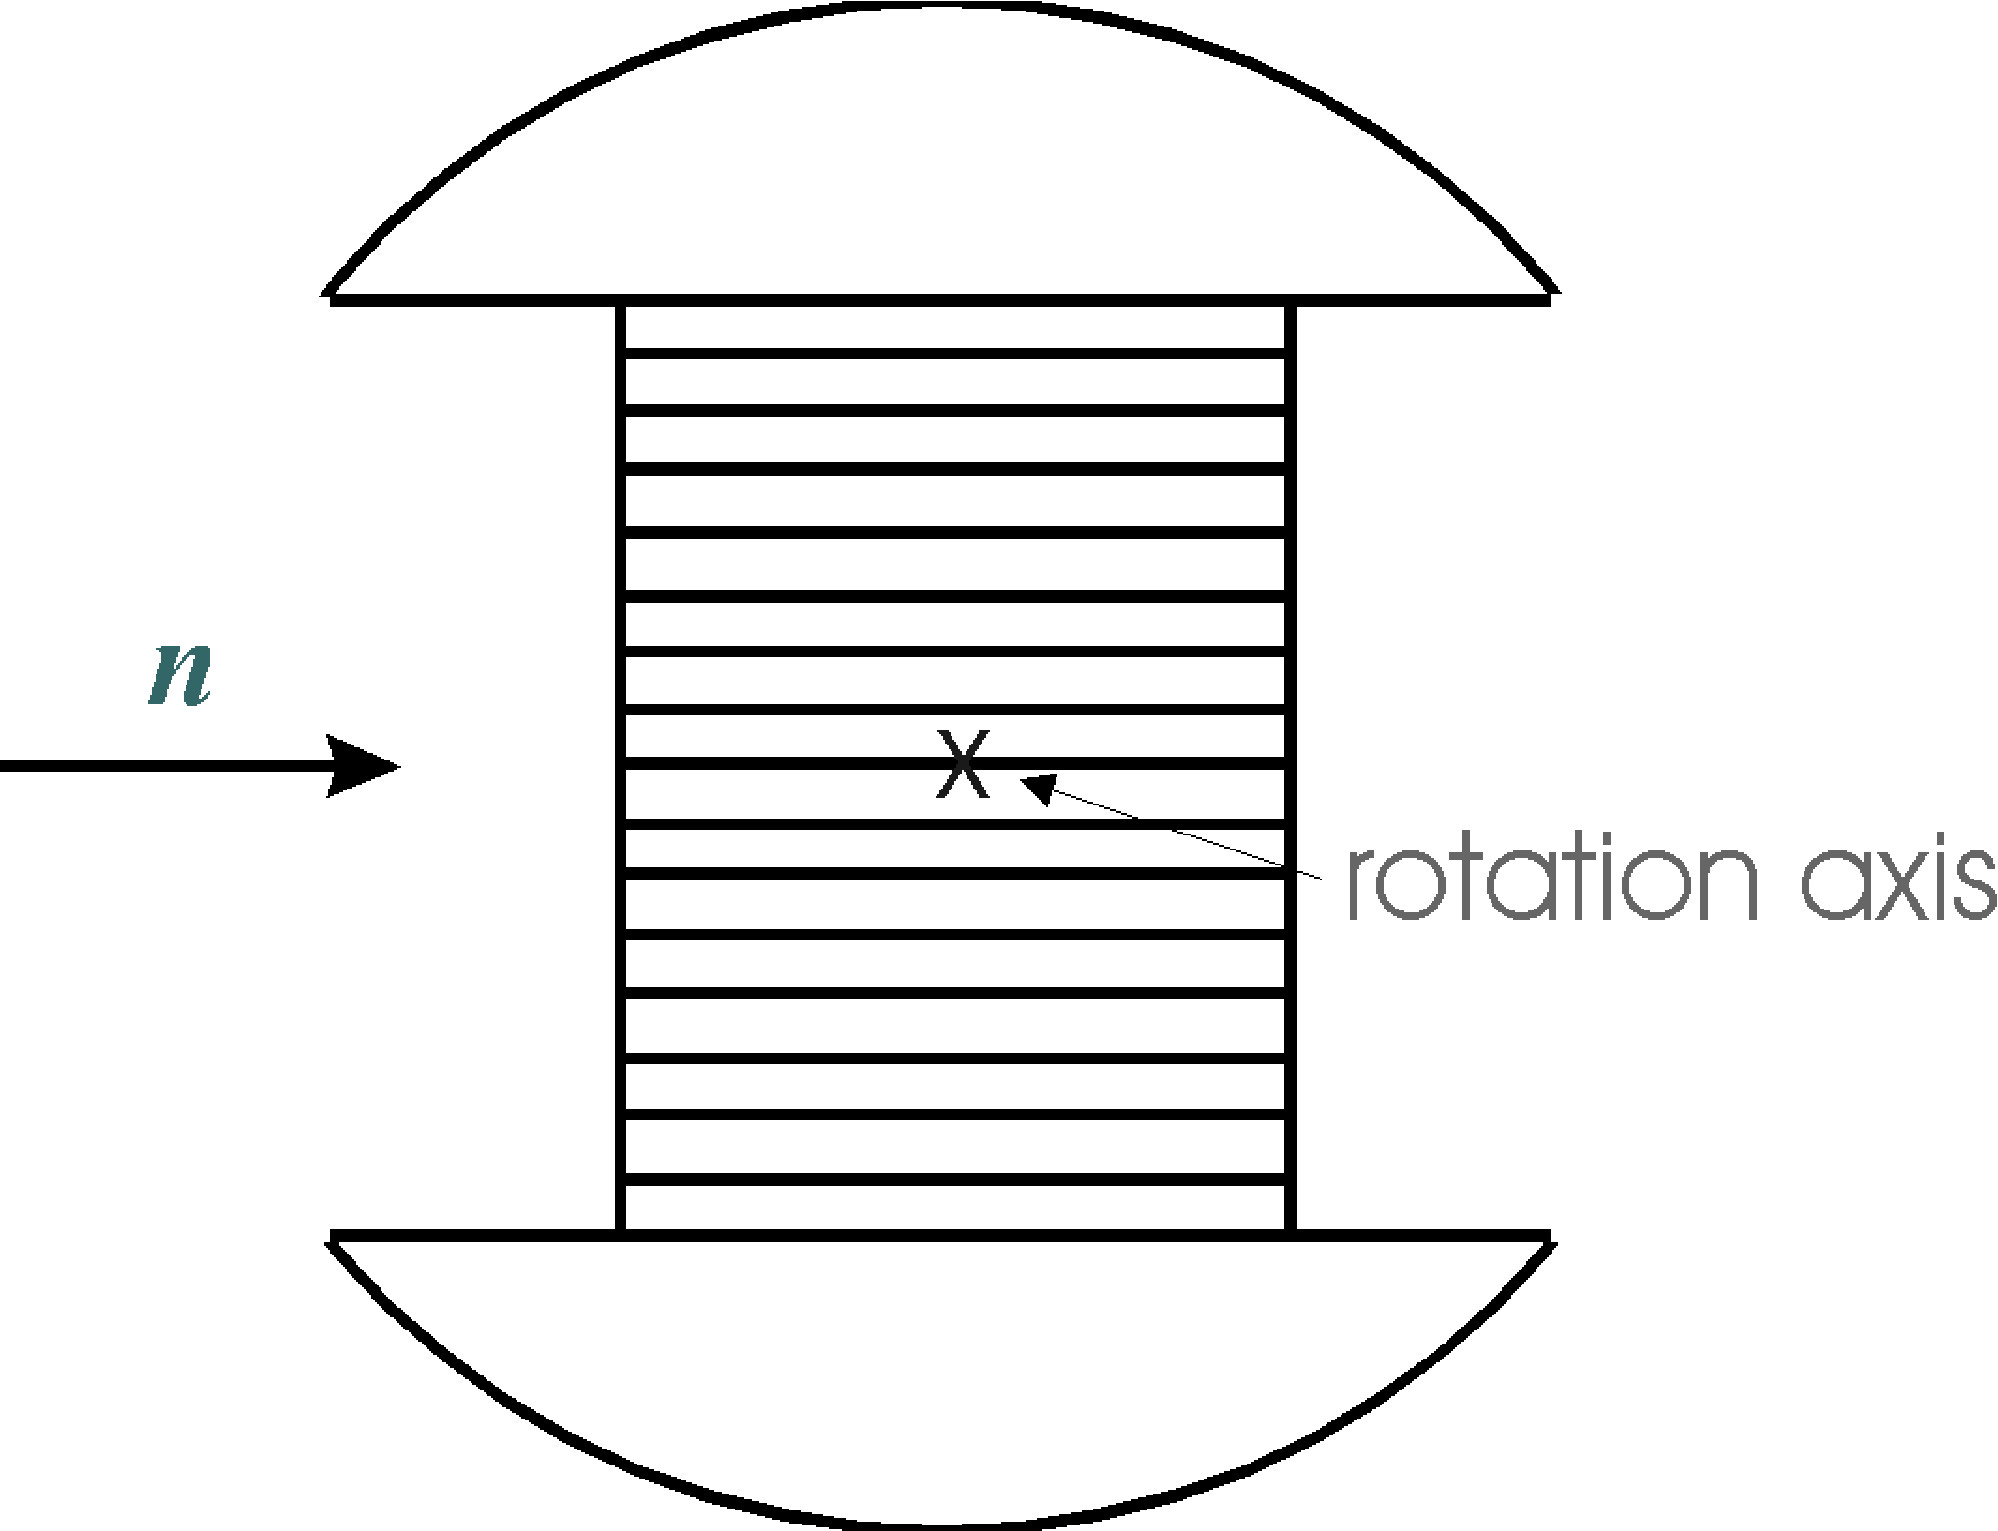
\includegraphics[width=0.45\linewidth]{figures/vitess_fc_str}
\caption{geometry of a staight Fermi chopper\label{f:vit_fc1}}
\end{center}
\end{figure}

Geometry for {\bf parabolic} channels:
In this case, the Fermi chopper is supposed to be a full cylinder, i.e. the central
channels are longer than those on the edges. The other features are the same as for
the other options. (see figure~\ref{f:vit_fc2}).

\begin{figure}[ht]
\begin{center}
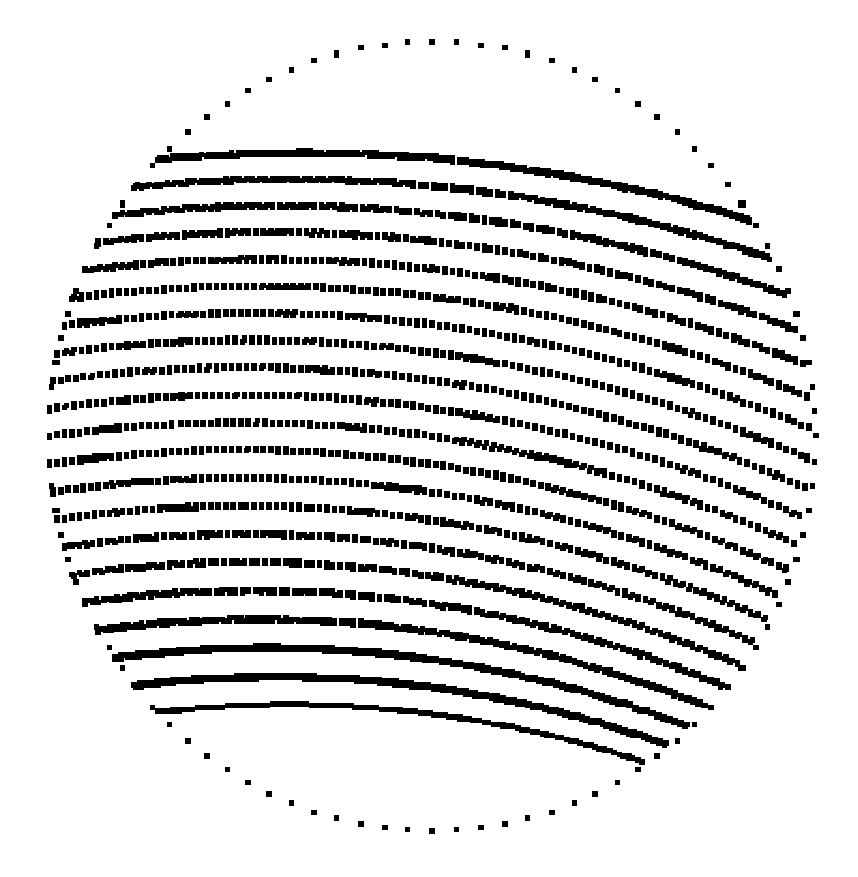
\includegraphics[width=0.4\linewidth]{figures/vitess_fc_parab}
\caption{geometry of a curved Fermi chopper\label{f:vit_fc2}}
\end{center}
\end{figure}

The algorithm works with a rotating chopper framework. Neutrons hitting the channel
walls are absorbed. The channels are approximated by $N_{\rm gates}$ gates. If the trajectory
takes a course through all the gates, the neutron passes the Fermi chopper. There are gates at
the entrance and the exit of the channel. The other gates are situated close to the centre of
the Fermic chopper.
Precision of the simulation increases with the number of gates, but also the computing time needed.
The use of four channels already gives exact transmission shapes for lower wavelengths
($\lambda < 6$ \AA) and good approximation for higher ones. It is recommended to use larger number of
channels only for a check.

The option 'zerotime' may be used to reset the time at the chopper position. The time is
set to a value between -$T_{\rm p}$/2 and +$T_{\rm p}$/2 (with $T_{\rm p}$ being the maximal pulse length),
depending on the phase of the chopper at the moment of passing the chopper centre. The
result is the generation of only 1 pulse instead of several; this is useful for TOF instruments
on continuous sources.

This component is about twice slower than the \verb+FermiChopper+ component.

The component must be placed after a component which sets a non zero flight path to the Fermi Chopper (e.g. not an Arm).


\newpage
\section{V\_selector: A rotating velocity selector}
\label{vselector}
\index{Optics!Velocity selector}

\component{V\_selector}{System}{$L_0$, $L_1$, $\omega$, $r_0$, $\phi$, $N$, height, width}{}{validated, position is center of input aperture}

\begin{figure}
  \begin{center}
    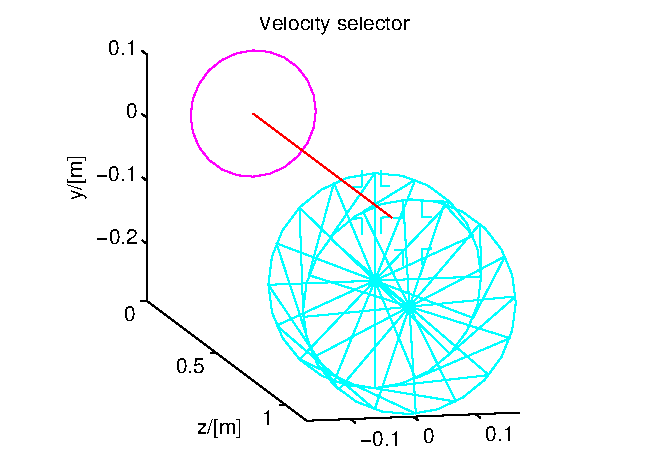
\includegraphics[width=0.9\textwidth]{figures/vselector}
  \end{center}
\caption{A velocity selector}
\label{f:vselector}
\end{figure}

The component {\bf V\_selector} models a rotating velocity
selector constructed from $N$ collimator blades
arranged radially on an axis. Two identical slits ($height \times width$)
at a 12 o'clock position allow
neutron passage at the position of the blades.
The blades are "twisted" on the axis so that a stationary
velocity selector does not transmit neutrons; the total
twist angle is denoted $\phi$ (in degrees).

Further input parameters for {\bf V\_selector} 
the distance between apertures, $L_0$, the length of the
collimator blades, $L_1$, the height from rotation axix to the slit
centre, $r_0$, the rotation speed $\omega$ (in rpm), 
and the blade thickness $t$.

The local coordinate system has its Origo at the slit centre.

The component {\rm Selector} produces equivalent results.

\subsection{Velocity selector transmission}

By rotating the selector you allow
transmittance of neutrons rays with velocities around a nominal value, given by
\begin{equation}
V_0 = \omega L / \phi ,
\end{equation}
which means that the selector has turned the twist angle
$\phi$ during the typical neutron flight time $L/V_0$. The actual twist angle
is $\phi' = \omega t = \omega L / V$.

Neutrons having a velocity slightly different from $V_0$
will either be transmitted or absorbed depending on the exact position
of the rotator blades when the neutron enters the selector.
Assuming this position to be unknown and integrating over all possible
positions (assuming zero thickness of blades), we arrive at a transmission factor
\begin{equation}
T = \left\{
 \begin{array}{ll}
 1 - (N/2\pi ) |\phi-\omega L / V| &
        {\rm if}\;   (N/2\pi )|\phi -\omega L / V| < 1 \\
    0  &  {\rm otherwise}
 \end{array} \right.
\end{equation}
where $N$ is the number of collimator blades.

A horisontal divergence changes the above formula because of the
angular difference between the entry and exit points of the neutron.
The resulting transmittance resembles the one above, only with
$V$ replaced by $V_z$ and $\phi$ replaced by $(\phi +\psi )$,
where $\psi$ is the angular difference due to
the divergence. An additional vertical divergence does not change
this formula, but it may contribute to $\psi$.
(We have here ignored the very small non-linearity of $\psi$ along the
neutron path in case of both vertical and horisontal divergence).

Adding the effect of a finite blade thickness, $t$, reduces the transmission
by the overall factor
\begin{equation}
\left( 1-\frac{N t}{2\pi r}  \right),
\end{equation}
where $r$ is the distance from the rotation axis. We ignore the variation
of $r$ along the neutron path and use just the average value.



\section{Selector: another approach to describe a rotating velocity selector}
\label{selector}
\index{Optics!Velocity selector}

\component{Selector}{System}{$xmin$, $xmax$, $ymin$, $ymax$, $len$, $num$, $width$, $radius$, $\alpha$, $feq$}{}{validated, position is center of input aperture}

The component {\bf Selector} describes the same kind of rotating velocity selector as {\bf V\_selector} - compare
description there - but it uses different parameters and a different algorithm:

The position of the apertures relative to the z-axis (usually the beam centre) is defined by the four parameters
$xmin, xmax, ymin, ymax$. Entry and exit apertures are always identical and situated directly before and behind
the rotor.
There are $num$ blades of thickness $width$ twisted by the angle $\alpha$ (in degrees) on a length $len$.
The selector rotates with a speed $feq$ (in rotation per second); its axle is in a distance $radius$ below the z-axis.

First the neutron is propagated to the entrance window. The loss of neutrons hitting the thin side
of the blades is taken into account by multiplying the neutron weight by a factor

\begin{equation}
   p(r) = \theta_i(r) / \theta_o
\end{equation}

\begin{equation}
   \theta_o = 360^o / num
\end{equation}

$\theta_i$ is the opening between two blades for the distance $r$ between the neutron position (at the entrance)
and the selector axle. The difference between $\theta_o$ and $\theta_i$ is determined by the blade thickness.
The neutron is now propagated to the exit window. If it is outside the regarded channel (between the two actual
blades), it is lost; otherwise it remains in the exit plane.

WARNING - Differences between {\bf Selector} and {\bf V\_selector}:
\begin{itemize}
\item {\bf Selector} has a different coordinate system than {\bf V\_selector};
in {\bf Selector} the origin lies in the entrance plane of the selector.
\item The blades are twisted to the other side, i.e. to the left above the axle in {\bf Selector}.
\item Speed of rotation is given in rotation per second, not in rotations per minute as in {\bf V\_selector}.
\end{itemize}





% there follows a chapter
\newpage
% Emacs settings: -*-mode: latex; TeX-master: "manual.tex"; -*-

\chapter{Monochromators}

In this class of components, we are concerned with elastic Bragg
scattering from monochromators. {\bf Monochromator\_flat}
models a flat thin mosaic crystal with a single scattering vector
perpendicular to the surface.
The component {\bf Monochromator\_curved} is physically similar,
but models a singly or doubly bend monochromator crystal arrangement.

A much more general model of scattering from a single crystal is
found in the component {\bf Single\_crystal},
which is presented under Samples, chapter~\ref{c:samples}.

\section{Monochromator\_flat: An infinitely thin, flat mosaic crystal with
a single scattering vector}
\label{s:monochromator_flat}
\index{Optics!Monochromator}

%\component{Monochromator\_flat}{System}{$z_{\rm min}$, $z_{\rm max}$, $y_{\rm min}$, $y_{\rm max}$, $\eta_{\rm h}$, $\eta_{\rm v}$, $R_0$, $Q_0$}{$d_{\rm m}$}{In reflecting geometry, non polarized}
\mcdoccomp{optics/Monochromator_flat.parms}

This component simulates an infinitely thin single
crystal with a single scattering vector, $Q_0=2\pi / d_m$, perpendicular to the
surface. A typical
use for this component is to simulate a simple monochromator or analyzer.

The monochromator dimensions are given by the length, $z_{\rm w}$, and
the height, $y_{\rm h}$. As the parameter names indicate, the
monochromator is placed in the $z-y$ plane of the local coordinate system.
This definition is made to ensure that the physical monochromator angle
(often denoted \verb+A1+) will equal the \MCS rotation angle
of the Monochromator component around the $y$-axis.
$R_0$ is the maximal reflectivity and
$\eta_{\rm h}$ and $\eta_{\rm v}$ are the horizontal and vertical mosaicities,
respectively, see explanation below.

\subsection{Monochromator physics and algorithm}
The physical model used in {\bf Monochromator\_flat} is a rectangular piece of
material composed of a large number of small micro-crystals.
The orientation of the
micro-crystals deviates from the nominal crystal orientation so that the
probability of a given micro-crystal orientation is proportional to a
Gaussian in the angle between the given and the nominal orientation. The
width of the Gaussian is given by the mosaic spread, $\eta$, of the crystal
(given in units of arc minutes).
$\eta$ is assumed to be large compared to the inherent Bragg width of the
scattering vector (often a few arc seconds).
(The mosaicity gives rise to a Gaussian reflectivity profile of width
similar to - but not equal - the intrinsic mosaicity.
In this component, and in real life, the mosaicity given is that of the
reflectivity signal.)

As a further simplification, the crystal is assumed to be infinitely
thin. This means that multiple scattering effects are not simulated. It
also means that the total reflectivity, $r_0$ is used as a parameter for
the model rather than the atomic scattering cross section, implying that
the scattering efficiency does not vary with neutron wavelength.
The variance
of the lattice spacing ($\Delta d/d$) is assumed to be zero, so this
component is not suitable for simulating backscattering instruments (use
the component {\rm Single\_crystal}
in section~\ref{s:Single_crystal} for that).

When a neutron trajectory intersects the crystal, the first step in the
computation is to determine the probability of scattering. This
probability is then used in a Monte Carlo choice deciding whether to
scatter or transmit the neutron. The physical scattering probability is the sum
of the probabilities of first- second-, and higher-order scattering -
up to the highest order possible for the given neutron wavelength.
However, in most cases at most one order will have a
significant scattering probability, and the computation thus considers
only the order that best matches the neutron wavelength.

The scattering of neutrons from a crystal is governed by Bragg's law:
\begin{equation}
n{\bf Q}_0 = 2{\bf k}_i\sin\theta
\end{equation}
The scattering order is specified by the integer $n$. We seek only one
value of $n$, namely the one which makes
$n {\bf Q}_0$ closest to the projection of $2{\bf k}_i$ onto ${\bf Q}_0$
(see figure~\ref{f:mosaic_order}).
%  k=2PI/lambda
%  q=2k sin(theta)
%
%  2 PI n/k = d q/2k
%  q = n 4 PI/d
%
%  n 2PI/k = n 4 PI/q \sin\theta
%  1/k = 2/q\sin\theta
%  n q = 2k\sin\theta
\begin{figure}
  \begin{center}
    \psfrag{theta}[l][l]{$\theta$}
    \psfrag{ki}[r][r]{$2{\bf k}_{\rm i}$}
    \psfrag{Q0}[l][l]{${\bf Q}_0$}
    \psfrag{2Q0}[l][l]{$2{\bf Q}_0$}
    \psfrag{3Q0}[l][l]{$3{\bf Q}_0$}
    \psfrag{4Q0}[l][l]{$4{\bf Q}_0$}
    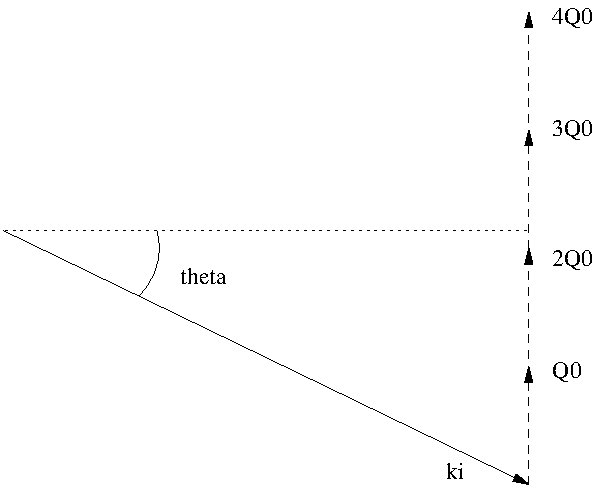
\includegraphics[width=0.5\textwidth]{figures/mosaic_order}
  \end{center}
\caption{Selection of the Bragg order (``2'' in this case).}
\label{f:mosaic_order}
\end{figure}
%

Once $n$ has been determined, the Bragg angle $\theta$ can be
computed. The angle $\alpha$ is the amount one would need to
turn the nominal scattering vector ${\bf Q}_0$ for the monochromator
to be in Bragg scattering condition.
We now use $\alpha$ to compute the probability of reflection from
the mosaic crystal
\begin{equation}
p_{\rm reflect} = R_0 e^{-\alpha^2/2\eta^2},
\end{equation}
The probability $p_{\rm reflect}$ is used
in a Monte Carlo choice to decide whether the neutron is transmitted or
reflected.
%
%\begin{figure}
%  \begin{center}
%    \psfrag{th}[r][r]{$\theta$}
%    \psfrag{ki}[r][r]{$2{\bf k}_{\rm i}$}
%    \psfrag{kf}[l][l]{$2{\bf k}_{\rm f}$}
%    \psfrag{Q0}[l][l]{${\bf Q}_0$}
%    \psfrag{alpha}[c][c]{$\alpha$}
%    \psfrag{q}[l][l]{$\bf q$}
%    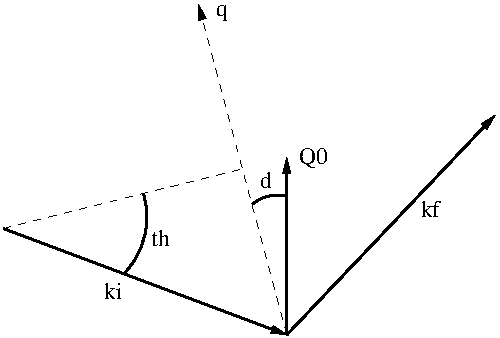
\includegraphics[width=0.5\textwidth]{figures/mosaic_angle}
%  \end{center}
%\caption{Computing the deviation $d$ from the nominal scattering direction.}
%\label{f:mosaic_angle}
%\end{figure}

In the case of reflection, the neutron will be scattered into the
Debye-Scherrer cone, with the probability of each point on the cone
being determined by the mosaic. The Debye-Scherrer cone can be described
by the equation
\begin{equation}
  \label{eq:mosaic_cone}
  {\bf k}_{\rm f} = {\bf k}_{\rm i}\cos2\theta +
      \sin2\theta({\bf c}\cos\varphi + {\bf b}\sin\varphi),
      \qquad\varphi\in[-\pi;\pi],
\end{equation}
where ${\bf b}$ is a vector perpendicular to ${\bf k}_{\rm i}$ and ${\bf
Q}_0$, ${\bf c}$ is perpendicular to ${\bf k}_{\rm i}$ and ${\bf b}$,
and both ${\bf b}$ and ${\bf c}$ have the same length as ${\bf k}_{\rm i}$
(see figure~\ref{f:mosaic_cone}). When choosing $\varphi$ (and
thereby ${\bf k}_{\rm f}$), only a small part of the full $[-\pi; \pi]$
range will have appreciable scattering probability in non-backscattering
configurations. The best statistics is thus obtained by sampling
$\varphi$ only from a suitably narrow range.

The (small) deviation angle $\alpha$ of the nominal
scattering vector $n{\bf Q}_0$ corresponds to a $\Delta q$ of
\begin{equation}
\Delta q \approx \alpha 2k\sin\theta.
\end{equation}
The angle $\varphi$ corresponds to a $\Delta k_{\rm f}$ (and hence
$\Delta q$) of
\begin{equation}
\Delta q \approx \varphi k \sin(2\theta)
\end{equation}
(see figure~\ref{f:mosaic_cone}).
Hence we may sample $\varphi$ from a Gaussian with standard deviation
\begin{equation}
\alpha\frac{2k\sin\theta}{k\sin(2\theta)} =
\alpha\frac{2k\sin\theta}{2k\sin\theta\cos\theta} =
\frac{\alpha}{\cos\theta}
\end{equation}
to get good statistics.
%
\begin{figure}
  \begin{center}
    \psfrag{th}[r][r]{$2\theta$}
    \psfrag{ki}[c][c]{$2{\bf k}_{\rm i}$}
    \psfrag{kf}[r][r]{$2{\bf k}_{\rm f}$}
    \psfrag{nQ0}[l][l]{$n{\bf Q}_0$}
    \psfrag{q}[l][l]{$\bf q$}
    \psfrag{2ksin2t}[l][l]{$2 k \sin(2 \theta)$}
    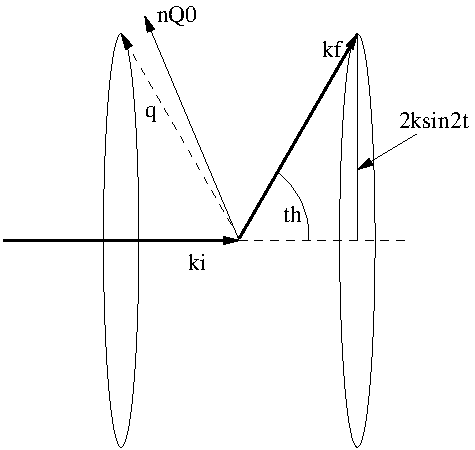
\includegraphics[width=0.5\textwidth]{figures/mosaic_cone}
  \end{center}
\caption{Scattering into the part of the Debye-Scherrer cone covered by
    the mosaic.}
\label{f:mosaic_cone}
\end{figure}

What remains is to determine the neutron weight. The distribution from
which the scattering event is sampled is a Gaussian in $\varphi$ of
width $\frac{\alpha}{\cos\theta}$,
\begin{equation}
    f_{\rm MC}(\varphi) = \frac{1}{\sqrt{2\pi}(\sigma/\cos\theta)}
            e^{-\varphi^2/2(\sigma/\cos\theta)^2}
\end{equation}
In the physical model, the probability of the scattering event is
proportional to a Gaussian in the angle between the nominal scattering
vector ${\bf Q}_0$ and the actual scattering vector ${\bf q}$. The
normalization condition is that the integral over all $\varphi$ should
be 1. Thus the probability of the scattering event in the physical model
is
\begin{equation}
  \label{eq:mosaic_integral}
  \Pi(\varphi) = e^{\frac{-d(\varphi)^2}{2\sigma^2}} /
   \int_{-\pi}^{\pi} e^{\frac{-d(\varphi)^2}{2\sigma^2}} d\varphi
\end{equation}
where $d(\varphi)$ denotes the angle between the nominal scattering
vector and the actual scattering vector corresponding to $\varphi$.
According to equation~(\ref{probrule}), the weight adjustment $\pi_j$ is
then given by
\begin{equation}
\pi_j = \Pi(\varphi) / f_{\rm MC}(\varphi).
\end{equation}
In the implementation, the integral in~(\ref{eq:mosaic_integral}) is computed
using a 15-order Gaussian quadrature formula, with the integral
restricted to an interval of width $5\sigma/\cos\theta$ for the same
reasons discussed above on the sampling of $\varphi$.


\section{Monochromator\_curved: A curved mosaic crystal with
a single scattering vector}
\label{s:monochromator_curved}
\index{Optics!Monochromator, curved}

%\component{Monochromator\_curved}{(System) Peter Link, FRM-2}{$z_{\rm w}$, $y_{\rm h}$, gap, $\eta_{\rm h}$, $\eta_{\rm v}$, $n_{\rm h}$, $n_{\rm v}$, $R_0$, $Q$, $r_{\rm h}$, $r_{\rm v}$}{$d_{\rm m}$, $\eta$, $h$, $w$, verbose, transmit, reflect}{In reflecting geometry, non polarized}
\mcdoccomp{optics/Monochromator_curved.parms}

\begin{figure}
  \begin{center}
    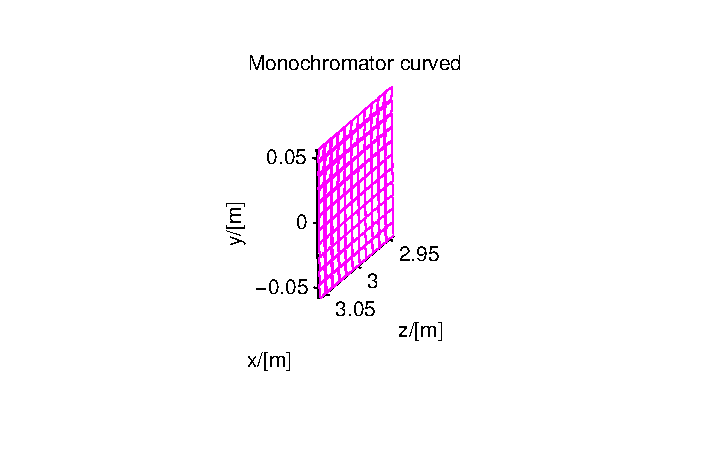
\includegraphics[width=0.9\textwidth]{figures/monochromator_curved}
  \end{center}
\caption{A curved monochromator}
\label{f:monochromator_curved}
\end{figure}


This component simulates an array of infinitely thin single
crystals with a single scattering vector perpendicular to the
surface and a mosaic spread.
This component is used to simulate a singly or doubly
curved monochromator or analyzer in reflecting geometry.

The component uses rectangular pieces of monochromator material
as described in {\bf Monochromator\_curved}.
The scattering vector is named $Q$, and as described in
{\bf Monochromator\_flat}, multiples of $Q$ will be applied.
Other important parameters are the piece height and width,
$y_{\rm h}$ and $z_{\rm w}$, respectively, the
horizontal and vertical mosaicities, $\eta_{\rm h}$ and $\eta_{\rm v}$,
respectively.
If just one mosaicity, $\eta$, is specified, this the same for both directions.

The number of pieces vertically and horizontally are called
$n_{\rm v}$ and $n_{\rm h}$, respectively, and the vertical and horizontal
radii of curvature are named $r_{\rm v}$ and $r_{\rm h}$, respectively.
All single crystals are positioned in the same vertical plane,
but tilted accordingly to the curvature radius.

The constant monochromator reflectivity, $R_0$ can be replaced by
a file of tabulated reflectivities $reflect$ (\verb+*.rfl+ in \verb+MCSTAS/data+). In the same sense, the transmission
can be modeled by a tabulated file $transmit$ (for non-reflected neutrons, \verb+*.trm+ in \verb+MCSTAS/data+).
The most useful of these files for Monochromator\_curved are \verb+HOPG.rlf+ and \verb+HOPG.trm+.

As for {\bf Monochromator\_flat}, the crystal is assumed to be infinitely
thin, and the variation in lattice spacing, ($\Delta d/d$),
is assumed to be zero. Hence, this
component is not suitable for simulating backscattering instruments or to
investigate multiple scattering effects.

The theory and algorithm for scattering from
the individual blades is described under {\bf Monochromator\_flat}.


\section{Single\_crystal: Thick single crystal monochromator plate with multiple scattering}
\index{Optics!Monochromator, thick}

The {\bf Single\_crystal} component may be used to study more complex monochromators, including incoherent scattering, thickness and multiple scattering. Please refer to section \ref{s:Single_crystal}.

\section{Phase space transformer - moving monochromator}
\index{Optics!phase space transformer}

Eventhough there exist a few attempts to write dedicated phase space transformer components, there is an elegant way to put a monochromator into move, by mean of the EXTEND keyword. If you define a SPEED parameter for the instrument, the idea is to change the coordinate system before the monochromator, and restore it afterwards, as follow in the TRACE section:
\begin{lstlisting}
DEFINE INSTRUMENT PST(SPEED=200, ...)
(...)
TRACE
(...)
COMPONENT Mono_PST_on=Arm()
AT ...
EXTEND %{
  vx = vx + SPEED; // monochromator moves transversaly by SPPED m/s
%}

COMPONENT  Mono=Monochromator(...)
AT (0,0,0) RELATIVE PREVIOUS

COMPONENT Mono_PST_off=Arm
AT (0,0,0) RELATIVE PREVIOUS
EXTEND  %{
  vz = vz - SPEED; // puts back neutron in static coordinate frame
%}
\end{lstlisting}
This solution does not contain acceleration, but is far enough for most
studies, and it is very simple. In the latter example, the instance \verb+Mono_PST_on+ should itself be rotated to reflect according to a Bragg law.

